\documentclass[12pt]{amsart}
\usepackage{amsmath,amssymb,amsthm}
\usepackage{geometry}                % See geometry.pdf to learn the layout options. There are lots.
\geometry{letterpaper}                   % \ldots or a4paper or a5paper or \ldots
%\geometry{landscape}                % Activate for for rotated page geometry
%\usepackage[parfill]{parskip}    % Activate to begin paragraphs with an empty line rather than an indent
\usepackage{graphicx}
\usepackage{amssymb}
\usepackage{epstopdf}
\usepackage{tikz}
\usepackage{pgfplots}
\usepackage{enumerate}
\usepackage{hyperref}
\DeclareGraphicsRule{.tif}{png}{.png}{`convert #1 `dirname #1`/`basename #1 .tif`.png}


\usepackage{mathtools}

\def\multichoose#1#2{\ensuremath{\left(\kern-.3em\left(\genfrac{}{}{0pt}{}{#1}{#2}\right)\kern-.3em\right)}}

\usepackage{verbatim}
%% Set up timestamp

%\usepackage[us,12hr]{datetime}





%\newcommand{\timestamp}{{\texttt{\currenttime , \today}}}

\hypersetup{
    colorlinks=true,
    linkcolor=blue,
    filecolor=magenta,      
    urlcolor=cyan,
    citecolor=red,
}
%\usepackage{lineno}
%\linenumbers


\newcommand{\ba}{\begin{enumerate}[(a)]}
\newcommand{\ea}{\end{enumerate}}



\newcommand{\bi}{\begin{enumerate}[(i)]}
\newcommand{\ei}{\end{enumerate}}




\definecolor{resred}{RGB}{214,0,23}
\def\check#1{{\color{resred}#1}}

%% A nice way to TeX sets
	\def\set#1{\left\{ {#1} \right\}}
	\def\setof#1#2{{\left\{#1 \mid #2\right\}}}
	\setlength{\textheight}{8.7truein}
%\setlength{\textwidth}{6.5truein}
%\setlength{\evensidemargin}{0truein}
%\setlength{\oddsidemargin}{0truein}
%\setlength{\topmargin}{0truein}
	
%% Some useful macros
	\def\Spec{\operatorname{Spec}}
	\def\Char{\operatorname{char}}
        \def\sdefect{\operatorname{sdefect}}
	\def\C{{\mathbb C}}
	\def\Z{{\mathbb Z}}
	%\def\F{{\mathbb F}}
	\def\bF{{\mathbb F}}
	\def\Q{{\mathbb Q}}
	\def\R{{\mathbb R}}
	\def\P{{\mathbb P}}
	\def\X{{\mathbb X}}
	\def\A{{\mathbb A}}
	\def\V{{\tilde{V}}}
	\def\mP{{\mathcal P}}
	\def\H{{\mathcal H}}
	\def\L{{\mathbb L}}
	\def\N{{\mathbb N}}
	\def\M{{M}}
	\def\sM{{M}}
	\def\B{{\mathcal B}}
	\def\E{{\mathcal E}}
	\def\cC{{\mathcal C}}
	\def\cD{{\mathcal D}}
	\def\O{{\mathcal O}}
	\def\I{{\mathcal I}}
	\def\sC{{\mathscr C}}
	\def\x{{\bold x}}
	\def\c{{1}}
	%\def\l{{\ell}}
	\def\y{{\bold y}}
	\def\field{{k}}
	\def\e{{\varepsilon}}
	\def\Span{{\text{span}}}
	\def\sing{{\text{Sing}}}
	\def\Ass{{\text{Ass}}}
	\def\satdeg{{\text{satdeg}}}
	\def\sat{{\text{sat}}}
	\def\reg{{\text{reg}}}
	\def\isomorphic{{\,\cong\,}}

\renewcommand{\geq}{\geqslant}
\renewcommand{\ge}{\geqslant}
\renewcommand{\leq}{\leqslant}
\renewcommand{\le}{\leqslant}


%% Setting up theorems

\theoremstyle{plain}

\newtheorem{theorem}{Theorem}[section]
\newtheorem{corollary}[theorem]{Corollary}
\newtheorem{proposition}[theorem]{Proposition}
\newtheorem{lem}[theorem]{Lemma}
%\newtheorem{claim}[thm]{Claim}
\newtheorem{ex}[theorem]{Example}

\theoremstyle{definition}

\newtheorem{example}[theorem]{Example}
%
%\newtheorem{exdefn}[thm]{Example/Definition}
\newtheorem{definition}[theorem]{Definition}
%\newtheorem{fact}[thm]{Fact}
%\newtheorem{conj}[thm]{Conjecture}
\newtheorem{question}[theorem]{Question}
%\newtheorem{notation}[thm]{Notation}
\newtheorem{remark}[theorem]{Remark}




%\newtheorem{innercustomthm}{Theorem}
%\newenvironment{customthm}[1]
%  {\renewcommand\theinnercustomthm{#1}\innercustomthm}
%  {\endinnercustomthm}
  
  
%\usepackage{mathpple}
%\renewenvironment{proof}[1][\proofname]{\begin{trivlist}\pushQED{\qed}\item[\hskip \labelsep  \bfseries #1{}.\hspace{10pt}]}
%{\popQED\end{trivlist}}
%\renewcommand{\qedsymbol}{$\blacksquare$}

%\pagestyle{fancyplain}
%\chead[\bigbf ]{\bigbf }
%\cfoot[\it ]{\it }
%
%\lhead[\thesection]{\leftmark}
%\rhead[\thesubsection]{\rightmark}

%\title{Symbolic Powers of Odd Cycle Edge Ideals}

\title{Comparing Powers of Edge Ideals}


\author{Mike Janssen}
\address{Mathematics/Statistics Department, Dordt College, Sioux Center, IA 51250, USA}
\email{mike.janssen@dordt.edu}

\author{Thomas Kamp}
\address{Mathematics/Statistics Department, Dordt College, Sioux Center, IA 51250, USA}
\email{thmskmp@dordt.edu}

\author{Jason Vander Woude}
\address{Department of Mathematics, University of Nebraska-Lincoln,
Lincoln, NE 68588-0130, USA}
\email{jasonvw@huskers.unl.edu}

%\date{May 30, 2017}                                           % Activate to display a given date or no date



\begin{document}



\maketitle

\begin{abstract}
	Given a nontrivial homogeneous ideal $I\subseteq k[x_1,x_2,\ldots,x_d]$, a problem of great recent interest has been the comparison of the $r$th ordinary power of $I$ and the $m$th symbolic power $I^{(m)}$.
	This comparison has been undertaken directly via an exploration of which exponents $m$ and $r$ guarantee the subset containment $I^{(m)}\subseteq I^r$ and asymptotically via a computation of the resurgence $\rho(I)$, a number for which any $m/r > \rho(I)$ guarantees $I^{(m)}\subseteq I^r$.
	Recently, a third quantity, the symbolic defect, was introduced; as $I^t\subseteq I^{(t)}$, the symbolic defect is the minimal number of generators required to add to $I^t$ in order to get $I^{(t)}$.
	
	We consider these various means of comparison when $I$ is the edge ideal of certain graphs by describing an ideal $J$ for which $I^{(t)} = I^t + J$.
	When $I$ is the edge ideal of an odd cycle, our description of the structure of $I^{(t)}$ yields solutions to both the direct and asymptotic containment questions, as well as a partial computation of the sequence of symbolic defects.
	%We also explore extensions of our methods to edge ideals of other graphs, including complete graphs.
\end{abstract}

%\keywords{symbolic power; monomial ideals; edge ideal; resurgence; graphs; odd cycle.}

%\ccode{2000 Mathematics Subject Classification: 13F20}


\section{Introduction}

%\subsection{Overview}

Let $k$ be an algebraically closed field, and $I$ a nonzero proper homogeneous ideal in $S = k[x_0,x_1,x_2,\ldots,x_N]$.
Recall that the $m$th symbolic power of $I$ is the ideal
\[
	I^{(m)} = S \cap \left(\bigcap\limits_{P\in \Ass(I)} I^m S_P\right).
\]
Over the last 10--15 years, the structure of $I^{(m)}$ has been an object of ongoing study; see, e.g., the recent survey \cite{2017DaoEtAl}.
One avenue for this study has been the examination of the relationship between $I^{(m)}$ and the well-understood algebraic structure of $I^r$, the $r$th ordinary power of $I$.
The naive context in which to examine this relationship is via subset containments, i.e., for which $m$ and $r$, $s$, and $t$ do we have $I^{(m)}\subseteq I^r$ and $I^{s} \subseteq I^{(t)}$?
In fact, this line of inquiry has been extremely productive.
It is straightforward to see that $I^s \subseteq I^{(t)}$ if and only if $s \ge t$, but determining which $r$ and $m$ give $I^{(m)} \subseteq I^r$ is more delicate.

Seminal results of Ein-Lazarsfeld-Smith and Hochster-Huneke \cite{2001:einlazarsfeldsmith,2002:hochsterhuneke-invent} established that for such ideals, $I^{(m)} \subseteq I^r$ if $m/r \ge N$.
Additional information about the ideal under consideration generally leads to tighter results (see, e.g., \cite{2014:boccicooperharbourne,2013:DenkertJanssen,2013:dumnicki}).
This phenomenon led to Bocci and Harbourne's introduction of a quantity known as the \emph{resurgence} of $I$, denoted $\rho(I)$; it is the least upper bound of the set $T = \setof{m/r}{I^{(m)}\not\subseteq I^r}$.
Thus, if $m/r > \rho(I)$, we have $I^{(m)}\subseteq I^r$.

Recently, Galetto, Geramita, Shin, and Van Tuyl introduced a new measure of the difference between $I^{(m)}$ and $I^m$ known as the symbolic defect.
Since $I^m\subseteq I^{(m)}$, the quotient $I^{(m)}/I^m$ is a finite $S$-module; thus, we let $\sdefect(I,m)$ denote the number of minimal generators of $I^{(m)}/I^m$ as an $S$-module.
This is known as the symbolic defect, and the symbolic defect sequence is the sequence $\set{\sdefect(I,m)}_{m\in\N}$.
In \cite{2016:galettogeramitavantuyl}, the authors study the symbolic defect sequences of star configurations in $\P^n_k$ and homogeneous ideals of points in $\P^2_k$.

Our work considers all these questions in the context of a class of edge ideals.
Let $G = (V,E)$ be a (simple) graph on the vertex set $V = \set{x_1,x_2,\ldots,x_n}$ with edge set $E$.
The edge ideal of $G$, introduced in \cite{Villarreal1990}, is the ideal $I(G)\subseteq R = k[x_1,x_2,\ldots,x_n]$ given by
\[
	I(G) = (\setof{x_i x_j}{\set{x_i, x_j}\in E}).
\]
That is, $I(G)$ is generated by the products of pairs of those variables between which are edges in $G$.

In \cite{1994:simisvasconcelosvillareal}, the authors establish that, for an edge ideal $I = I(G)$, we have $I^{(m)} = I^m$ for all $m \ge 1$ if and only if $G$ is bipartite.
A natural question, then, is to explore the relationship between $I(G)^{(m)}$ and $I(G)^r$ when $G$ is not bipartite, which is equivalent to $G$ containing an odd cycle.
Thus, \cite{2004:worthenelliswilson} sought to explore this relationship when $G = C_{2n+1}$ is a cycle on $2n+1$ vertices.



We continue the problem of exploring the structure of the symbolic power $I(G)^{(t)}$ for certain classes of graphs $G$, with a focus on when $G$ is an odd cycle.
The main results of this work are Theorem \ref{lem:tl<it} and Corollary \ref{thm:sorta}, which together describe a decomposition of the form $I^{(t)} = I^t + J$, where $J$ is a well-understood ideal. 
We are then able to use this decomposition to resolve  \cite[Conjecture 15]{2004:worthenelliswilson}, compute $\rho(I(C_{2n+1}))$ in Theorem \ref{thm:resurgence}, and establish a partial symbolic defect sequence in Theorem \ref{thm:sdefects}.
We close by showing that our ideas in Theorem \ref{lem:tl<it} apply for complete graphs and graphs which consist of an odd cycle plus an additional vertex and edge.





\subsection*{Remark}
	As preparation of this manuscript was concluding in summer 2017, Dao et.~al posted the preprint \cite{2017DaoEtAl}.
	In particular, their Theorem 4.13 bears a striking resemblance to our Corollary \ref{cor:ordsymequal}. 
	While these similarities are worth noting, in part as evidence that interest in symbolic powers is high, it is also worth noting that the aims of these two works are distinct and complementary. 
	The aim of the relevant sections of  \cite{2017DaoEtAl} is to investigate the packing property for edge ideals, while ours is to more directly describe the difference between the ordinary and symbolic powers by investigating the structure of a set of minimal generators for $I^{(t)}$.
	We then use information about these generators to compute invariants related to the containment $I^{(m)}\subseteq I^r$.











\section{Background results}


Edge ideals are an important class of examples of squarefree monomial ideals, i.e., an ideal generated by elements of the form $x_1^{a_1} x_2^{a_2} \cdots x_n^{a_n}$, where $a_i \in \set{0,1}$ for all $i$.
When $I$ is squarefree monomial, it is well-known that the minimal primary decomposition is
\[
	I = P_1 \cap \cdots \cap P_r, \text{ with } P_j = (x_{j_1}, \ldots, x_{j_{s_j}}) \text{ for } j = 1, \ldots, r.
\]
When $I = I(G)$ is an edge ideal, the variables in the $P_j$'s are precisely the vertices in the minimal vertex covers of $G$.
Recall that, given a graph $G = (V,E)$, a \emph{vertex cover} of $G$ is a subset $V'\subseteq V$ such that for all $e\in E$, $e\cap V' \ne \emptyset$.
A \emph{minimal vertex cover} is a vertex cover minimal with respect to inclusion.
%The minimal vertex covers will be especially useful to us, as they describe the variables needed to decompose an edge ideal into its minimal primes (see, e.g., ).



\begin{lem}[\cite{VanTuyl2013}, Corollary 3.35]\label{lem:minprimevertexcover}
	Let $G$ be a graph on the vertices $\set{x_1,x_2,\ldots,x_n}$, $I = I(G) \subseteq k[x_1,x_2,\ldots,x_n]$ be the edge ideal of $G$ and $V_1, V_2, \ldots, V_r$ the minimal vertex covers of $G$.
	Let $P_j$ be the monomial prime ideal generated by the variables in $V_j$.
	Then
	\[
		I = P_1 \cap P_2 \cap \cdots \cap P_r
	\]
	and
	\[
		I^{(m)} = P_1^m \cap P_2^m \cap \cdots \cap P_r^m.
	\]
\end{lem}

Symbolic powers of squarefree monomial ideals (and, more specifically, edge ideals) have enjoyed a great deal of recent interest (see, e.g., \cite{2013:cooperembreehahoefel,2016:BocciMFO}).
In \cite{2016:BocciMFO}, a linear programming approach is used to compute invariants related to the containment question.
We adapt this technique in Lemma \ref{lem:alphasubprog} for the edge ideals under consideration in this paper.
One result of \cite{2016:BocciMFO} which will be of use is the following. %, which reduces the problem of determining whether a given monomial is in $I^{(m)}$ to a problem of checking certain (linear) constraints on the exponents of the variables.


\begin{lem}\label{lem:jdef}
Let $I \subseteq R$ be a squarefree monomial ideal with minimal primary decomposition $I = P_1 \cap P_2 \cap \cdots \cap P_r$ with $P_j = ( x_{j_1},\ldots,x_{j_{s_j}} )$ for $j = 1,\ldots,r$. Then
$x_{a_1}\cdots x_{a_n} \in I^{(m)}$ if and only if $a_{j_1}+\ldots+a _{j_{s_j}} \geq m$ for $j=1,\ldots,r$.
\end{lem}

%Note that this reduces the problem of determining whether a given monomial is in $I^{(m)}$ to checking conditions on the exponents of the variables.



\begin{remark}
	Throughout this work, we will be exploring questions about ideals in $R = k[x_1,x_2,\ldots,x_n]$ related to graphs on the vertex set $\set{x_1,x_2,\ldots,x_n}$.
	We will use the $x_i$'s interchangeably to represent both vertices and variables.
	The specific use should be clear from the context, and we see this as an opportunity to emphasize the close connection between the graph and the ideal.
\end{remark}





%\begin{definition}
%Edge ideal of cycle?
%\end{definition}


%\begin{definition}\label{def:i2t}
%definition of $I^t$?
%\end{definition}

%\begin{definition}
%original definitions of $I^{(t)}$?
%\end{definition}




%\begin{theorem}
%Known relationships between $I^{(t)}$ and $I^t$?
%\end{theorem}




\section{Factoring monomials along odd cycles}

In this section, we introduce the main ideas of our approach to studying symbolic powers of edge ideals.
We define a means of writing a monomial in a power of an edge ideal with respect to the minimal vertex covers of the graph and study the properties of this representation.
%We then study this representation. % and describe a situation in which it is not optimal.
In what follows, let $R = k[x_1,x_2,\ldots,x_{2n+1}]$ and let $I = I(C_{2n+1})$ be the edge ideal of the odd cycle $C_{2n+1}$. %, i.e., 
%\[
%	I = (x_1 x_2, x_2 x_3, \ldots, x_{2n} x_{2n+1}, x_{2n+1} x_1).
%\]




\begin{definition}\label{defn:optimal}
Let $m\in k[x_1,x_2,\ldots,x_{2n+1}]$ be a monomial.
	Let $e_j$ denote the monomial representing the $j$th edge in the cycle, i.e., $e_j = x_j x_{j+1}$ for $1\le j \le 2n$, and $e_{2n+1} = x_{2n+1} x_1$.
	We may then write 
	$$
		m = x_1^{a_1} x_2^{a_2} \cdots x_{2n+1}^{a_{2n+1}} e_1^{b_1} e_2^{b_2} \cdots e_{2n+1}^{b_{2n+1}},
	$$
	where $b(m) := \sum b_j$ is as large as possible (observe $0\le 2b(m) \le \deg(m)$) and $a_i \ge 0$. 
	When $m$ is written in this way, we will call this an \emph{optimal factorization} of $m$, or say that $m$ is expressed in \emph{optimal form}. In addition, each $x_i^{a_i}$ with $a_i > 0$ in this form will be called an \emph{ancillary factor} of the optimal factorization, or just an \emph{ancillary} for short.
\end{definition}

%% \begin{definition}\label{defn:optimal}
%% Let $m\in k[x_1,x_2,\ldots,x_{2n+1}]$ be a monomial.
%% Let $e_{i,j}$ denote the degree two monomial representing $x_i\cdot x_j$ and require that $i<j$. For cycles, let $e_i$ denote $e_{i,i+1}$ and $b_i$ denote $b_{i,i+1}$ for $1\le i \le 2n$, and $e_{2n+1} = e_{1,2n+1}$, $b_{2n+1} = b_{1,2n+1}$.
%% We may then write
%% $$m = x_1^{a_1} x_2^{a_2} \cdots x_{2n+1}^{a_{2n+1}} e_{1,2}^{b_{1,2}} e_{1,3}^{b_{1,3}} \cdots e_{2n,2n+1}^{b_{2n,2n+1}}$$
%% or for cycles
%% $$m = x_1^{a_1} x_2^{a_2} \cdots x_{2n+1}^{a_{2n+1}} e_1^{b_1} e_2^{b_2} \cdots e_{2n+1}^{b_{2n+1}}$$
%% 	where $b(m) := \sum b_j$ is as large as possible (observe $0\le 2b(m) \le \deg(m)$) and $a_i \ge 0$. 
%% 	When $m$ is written in this way, we will call this an \emph{optimal factorization} of $m$, or say that $m$ is expressed in \emph{optimal form}. In addition, each $x_i^{a_i}$ with $a_i > 0$ in this form will be called an \emph{ancillary factor} of the optimal factorization, or just an ancillary for short.
%% \end{definition}

Observe that the optimal form representation of $m$ is not unique in the sense that different edges may appear as factors of $m$; for example, in $k[x_1,\ldots,x_5]$, if $m = x_1^2 x_2^2 x_3 x_4 x_5$ we may write $m = x_1 e_1 e_2 e_4 = x_2 e_1 e_3 e_5$.



\begin{lem}\label{lem:splitm}
Let $m = x_1^{a_1} x_2^{a_2} \cdots x_{2n+1}^{a_{2n+1}} e_1^{b_1} e_2^{b_2} \cdots e_{2n+1}^{b_{2n+1}} \in I(C_{2n+1})$ be an optimal factorization. %, where $m \in I(C_{2n+1})$.
Then any $m' =  x_1^{a'_1} x_2^{a'_2} \cdots x_{2n+1}^{a'_{2n+1}} e_1^{b'_1} e_2^{b'_2} \cdots e_{2n+1}^{b'_{2n+1}}$ will also be an optimal factorization if $0 \leq a'_i \leq a_i$ and $0 \leq b'_j \leq b_j$ for all $i$ and $j$.
\end{lem}

\begin{proof}
Let $m' =  x_1^{a'_1} x_2^{a'_2} \cdots x_{2n+1}^{a'_{2n+1}} e_1^{b'_1} e_2^{b'_2} \cdots e_{2n+1}^{b'_{2n+1}}$ such that for all $i,j$, $0 \leq a'_i \leq a_i$ and $0 \leq b'_j \leq b_j$. 
Since each exponent of $m'$ is less than or equal to the corresponding exponent from $m$, we know that $m'$ divides $m$. 
Thus, there must exist some 
\[
	m'' = x_1^{(a_1-a'_1)} x_2^{(a_2-a'_2)} \cdots x_{2n+1}^{(a_{2n+1}-a'_{2n+1})} e_1^{(b_1-b'_1)} e_2^{(b_2-b'_2)} \cdots e_{2n+1}^{(b_{2n+1}-b'_{2n+1})}
\] 
such that $m = m'm''$.

Suppose that $m'$ is not in optimal form. 
Then we can re-express $m'$ as 
\[
m'=x_1^{c_1} x_2^{c_2} \cdots x_{2n+1}^{c_{2n+1}} e_1^{d_1} e_2^{d_2} \cdots e_{2n+1}^{d_{2n+1}},
\] 
such that $\sum b'_i < \sum d_i$. 
As $$m = m'm'' = \prod  x_i^{(a_i-a'_i+c_i)} e_i^{(b_i-b'_i+d_i)},$$ $m$ has an edge exponent sum of $\sum (b_i-b'_i+d_i) = \sum b_i - \sum b'_i + \sum d_i$. 
As $\sum b'_i < \sum d_i$, it must be true that $ \sum (b_i-b'_i+d_i) > \sum b_i$.

\end{proof}

The next lemma describes a process that will be critical in the proof of Theorem \ref{lem:it<tl}.
Intuitively, it says that if a monomial is factored along a path of an odd number of consecutive edges with ancillaries on both ends of this path of edges, the monomial is not written in optimal form, i.e., it can be rewritten as a product of strictly more edges.
Before stating and proving the lemma, we illustrate the process with an example.

\begin{example}\label{ex:first}
Let $G$ be a cycle with 111 vertices %\footnote{The reason why $G$ has 111 vertices is to emphasize that no potential edge exists between $x_1$ and $x_8$ and to suggest that this could just be one component of a much larger monomial.}  
and consider $m = x_1^3 x_2^4 x_3^2 x_4^3 x_5^5 x_6^3 x_7^2 x_8^2\in I(G)$ with edge factorization: $$m = x_1  e_1^2 e_2^2 e_4^3 e_5^2 e_6 e_7 x_8$$ where  $e_i = x_i x_{i+1}$. Note that in this factorization, there is an ancillary at $x_1$ and $x_8$. We will show that $m$ is not in optimal form.

We can graphically represent $m$ by drawing an edge between $x_i$ and $x_{i+1}$ for each $e_i$ in $m$ and creating a bold outline for each ancillary, as shown below:


\begin{center}
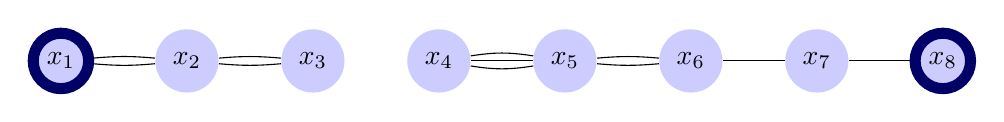
\begin{tikzpicture}[scale=1.6,auto=left,every node/.style={circle,fill=blue!20,inner sep=4}]
	\node[draw=blue!40!black,line width=4,inner sep=3pt] (n1) at (0,  0) {$x_1$};
	\node (n2) at (1,  0)  {$x_2$};
	\node (n3) at (2, 0)  {$x_3$};
	\node (n4) at (3, 0) {$x_4$};
	\node (n5) at (4,  0)  {$x_5$};
	\node (n6) at (5,  0)  {$x_6$};
	\node (n7) at (6,  0)  {$x_7$};
	\node[draw=blue!40!black,line width=4,inner sep=3pt]  (n8) at (7,  0)  {$x_8$};
  \draw (n1) to [bend right = -5] (n2);
  \draw (n1) to [bend right = 5] (n2);
  \draw (n2) to [bend right = 5] (n3);
  \draw (n2) to [bend right = -5] (n3);
  \draw (n4) to [bend right = -9] (n5);
  \draw (n4) to [bend right = 0] (n5);
  \draw (n4) to [bend right = 9] (n5);
  \draw (n7) to [bend right = 0] (n6);
  \draw (n6) to [bend right = -5] (n5);
  \draw (n6) to [bend right = 5] (n5);
  \draw (n7) to [bend right = 0] (n8);
\end{tikzpicture}
\end{center}

Using a method described more fully in Lemma \ref{lem:evens}, we will ``break'' each of the red (bolded) edges back into standard $x_i$ notation so that we create new ancillaries at every vertex.

\begin{center}
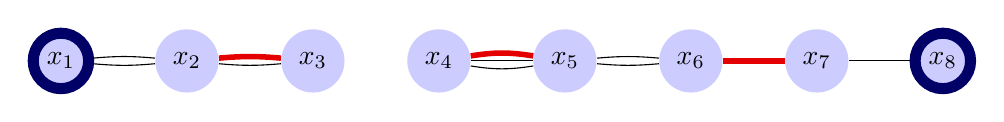
\begin{tikzpicture}[scale=1.6,auto=left,every node/.style={circle,fill=blue!20,inner sep=4}]
	\node[draw=blue!40!black,line width=4,inner sep=3pt] (n1) at (0,  0) {$x_1$};
	\node (n2) at (1,  0)  {$x_2$};
	\node (n3) at (2, 0)  {$x_3$};
	\node (n4) at (3, 0) {$x_4$};
	\node (n5) at (4,  0)  {$x_5$};
	\node (n6) at (5,  0)  {$x_6$};
	\node (n7) at (6,  0)  {$x_7$};
	\node[draw=blue!40!black,line width=4,inner sep=3pt]  (n8) at (7,  0)  {$x_8$};
  \draw (n1) to [bend right = -5] (n2);
  \draw (n1) to [bend right = 5] (n2);
  \draw (n2) to [bend right = 5] (n3);
  \draw[red!90!black, line width = 2] (n2) to [bend right = -5] (n3);
  \draw[red!90!black, line width = 2] (n4) to [bend right = -9] (n5);
  \draw (n4) to [bend right = 0] (n5);
  \draw (n4) to [bend right = 9] (n5);
  \draw[red!90!black, line width = 2] (n7) to [bend right = 0] (n6);
  \draw (n6) to [bend right = -5] (n5);
  \draw (n6) to [bend right = 5] (n5);
  \draw (n7) to [bend right = 0] (n8);
\end{tikzpicture}


\begin{tikzpicture}[fill=black,ultra thick, scale = .22, transform shape,font=\Large]
\draw [fill = black] (.3,1) -- (2.7,1) -- (1.5,0) -- cycle;
\draw [fill = black] (1,1) -- (2,1) -- (2,2) -- (1,2) -- cycle;
\end{tikzpicture}

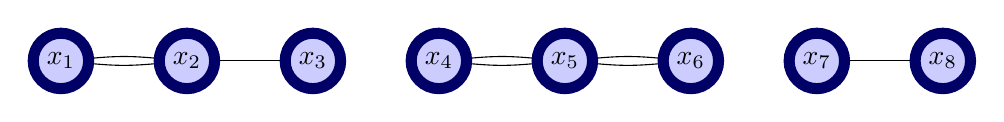
\begin{tikzpicture}[scale=1.6,auto=left,every node/.style={circle,fill=blue!20,draw=blue!40!black,line width=4,inner sep=3pt}]
	\node (n1) at (0,  0) {$x_1$};
	\node (n2) at (1,  0)  {$x_2$};
	\node (n3) at (2, 0)  {$x_3$};
	\node (n4) at (3, 0) {$x_4$};
	\node (n5) at (4,  0)  {$x_5$};
	\node (n6) at (5,  0)  {$x_6$};
	\node (n7) at (6,  0)  {$x_7$};
	\node  (n8) at (7,  0)  {$x_8$};
  \draw (n1) to [bend right = -5] (n2);
  \draw (n1) to [bend right = 5] (n2);
  \draw (n2) to [bend right = 0] (n3);
  \draw (n4) to [bend right = -5] (n5);
  \draw (n4) to [bend right = 5] (n5);
  \draw (n6) to [bend right = -5] (n5);
  \draw (n6) to [bend right = 5] (n5);
  \draw (n7) to [bend right = 0] (n8);
\end{tikzpicture}
\end{center}

Note that if we define a new monomial $p$ based on this graphical representation, where $p = x_1 x_2 x_3 x_4 x_5 x_6 x_7 x_8 e_1^2 e_2 e_4^2 e_5^2 e_7$, we have $m = p$ because we are merely changing the factorization of the monomial $m$, not its value.

As one can see, there are now 8 consecutive ancillaries, which we can pair up in a new way, as shown below. New edges are  highlighted in green (bolded in the second line).

\begin{center}
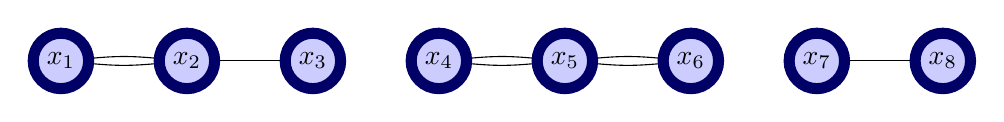
\begin{tikzpicture}[scale=1.6,auto=left,every node/.style={circle,fill=blue!20,draw=blue!40!black,line width=4,inner sep=3pt}]
	\node (n1) at (0,  0) {$x_1$};
	\node (n2) at (1,  0)  {$x_2$};
	\node (n3) at (2, 0)  {$x_3$};
	\node (n4) at (3, 0) {$x_4$};
	\node (n5) at (4,  0)  {$x_5$};
	\node (n6) at (5,  0)  {$x_6$};
	\node (n7) at (6,  0)  {$x_7$};
	\node  (n8) at (7,  0)  {$x_8$};
  \draw (n1) to [bend right = -5] (n2);
  \draw (n1) to [bend right = 5] (n2);
  \draw (n2) to [bend right = 0] (n3);
  \draw (n4) to [bend right = -5] (n5);
  \draw (n4) to [bend right = 5] (n5);
  \draw (n6) to [bend right = -5] (n5);
  \draw (n6) to [bend right = 5] (n5);
  \draw (n7) to [bend right = 0] (n8);
\end{tikzpicture}


\begin{tikzpicture}[fill=black,ultra thick, scale = .22, transform shape,font=\Large]
\draw [fill = black] (.3,1) -- (2.7,1) -- (1.5,0) -- cycle;
\draw [fill = black] (1,1) -- (2,1) -- (2,2) -- (1,2) -- cycle;
\end{tikzpicture}

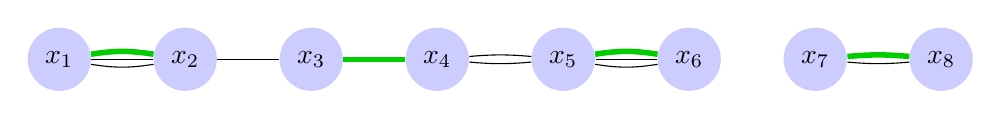
\begin{tikzpicture}[scale=1.6,auto=left,every node/.style={circle,fill=blue!20,inner sep=4}]
	\node (n1) at (0,  0) {$x_1$};
	\node (n2) at (1,  0)  {$x_2$};
	\node (n3) at (2, 0)  {$x_3$};
	\node (n4) at (3, 0) {$x_4$};
	\node (n5) at (4,  0)  {$x_5$};
	\node (n6) at (5,  0)  {$x_6$};
	\node (n7) at (6,  0)  {$x_7$};
	\node (n8) at (7,  0)  {$x_8$};
  \draw[green!80!black, line width = 2] (n1) to [bend right = -9] (n2);
  \draw (n1) to [bend right = 9] (n2);
  \draw (n1) to [bend right = 0] (n2);
  \draw (n2) to [bend right = 0] (n3);
  \draw[green!80!black, line width = 2] (n3) to [bend right = 0] (n4);
  \draw (n4) to [bend right = -5] (n5);
  \draw (n4) to [bend right = 5] (n5); 
  \draw[green!80!black, line width = 2] (n6) to [bend right = 9] (n5);
  \draw (n6) to [bend right = -9] (n5);
  \draw (n6) to [bend right = 0] (n5);
  \draw[green!80!black, line width = 2] (n7) to [bend right = -5] (n8);
  \draw (n7) to [bend right = 5] (n8);
\end{tikzpicture}
\end{center}

Now we have a third possible representation $q$ of this monomial. Note that $q = e_1^3 e_2 e_3 e_4^2 e_5^3 e_7^2$ and $q=p=m$. As you can see, this monomial representation has one more edge than our original representation, which means that $m$ is not optimal.
\end{example}

\begin{lem}\label{lem:evens}
Let $m = x_j^{a_j} e_j^{b_j} e_{j+1}^{b_{j+1}} \cdots e_{j+2k}^{b_{j+2k}} x_{j+2k+1}^{a_{j+2k+1}}$, where $a_j, a_{j+2k+1} \geq 1$. If it is the case that $b_{j+2h+1} \geq 1$ for all $h \in \{0,\ldots,k-1\}$, then $m$ is not in optimal form.
\end{lem}

\begin{proof}
Let $m = x_j^{a_j} e_j^{b_j} e_{j+1}^{b_{j+1}} \cdots e_{j+2k}^{b_{j+2k}} x_{j+2k+1}^{a_{j+2k+1}}$ and notice that $m$ is a string of adjacent edges with ancillaries on either end. We will show that this representation of $m$ is not optimal. % by making use of the existence of alternating edges.
For clarity, and without loss of generality, let $j=1$, and suppose that $b_i \geq 1$ for all evenly indexed edge exponents. 

Let $p = x_1 e_2 e_{4} \cdots e_{2k} x_{2k+2}$ and note that %let $q = x_1^{(a_{1} - 1)} e_1^{b_1} e_{2}^{(b_{2} - 1)} \cdots e_{2k+1}^{b_{2k+1}} x_{2k+2}^{(a_{2k+2}-1)}$ so that $m = pq$.
by Lemma \ref{lem:splitm}, $p$ must be in optimal form if $m$ is expressed optimally. However, 
\begin{align*}
p &= 
x_1 e_2 e_{4} \cdots e_{2k} x_{2k+2} \\
&= x_1(x_2 x_3) (x_4 x_5) \cdots (x_{2k} x_{2k+1}) x_{2k+2} \\
&= (x_1x_2) (x_3 x_4) (x_5 x_6) \cdots (x_{2k+1} x_{2k+2}) \\
&= e_1 e_3 e_5  \cdots e_{2k+1}.
\end{align*}
%Since $p$ was not initially expressed in optimal form, we know that $m$ could not have been an optimal factorization.
\end{proof}

%%%%%%%%%%%%%%%%%%%%%%%%%%%%%%%%%%%%%%%
%%%%%%%%%%%%%%%%%%%%%%%%%%%%%%%%%%%%%%%
%%%%%%%%%%%%%%%%%%%%%%%%%%%%%%%%%%%%%%%
%%%%%%%%%%%%%%%%%%%%%%%%%%%%%%%%%%%%%%%
%%%%%%%%%%%%%%%%%%%%%%%%%%%%%%%%%%%%%%%
%%%%%%%%%%%%%%%%%%%%%%%%%%%%%%%%%%%%%%%
%%%%%%%%%%%%%%%%%%%%%%%%%%%%%%%%%%%%%%%
%%%%%%%%%%%%%%%%%%%%%%%%%%%%%%%%%%%%%%%



%%%%%%%%%%%%%%%%%%%%%%%%%%%%%%%%%%%%%%%
%%%%%%%%%%%%%%%%%%%%%%%%%%%%%%%%%%%%%%%
%%%%%%%%%%%%%%%%%%%%%%%%%%%%%%%%%%%%%%%
%%%%%%%%%%%%%%%%%%%%%%%%%%%%%%%%%%%%%%%
%%%%%%%%%%%%%%%%%%%%%%%%%%%%%%%%%%%%%%%
%%%%%%%%%%%%%%%%%%%%%%%%%%%%%%%%%%%%%%%
%%%%%%%%%%%%%%%%%%%%%%%%%%%%%%%%%%%%%%%
%%%%%%%%%%%%%%%%%%%%%%%%%%%%%%%%%%%%%%%



%%%%%%%%%%%%%%%%%%%%%%%%%%%%%%%%%%%%%%%
%%%%%%%%%%%%%%%%%%%%%%%%%%%%%%%%%%%%%%%
%%%%%%%%%%%%%%%%%%%%%%%%%%%%%%%%%%%%%%%
%%%%%%%%%%%%%%%%%%%%%%%%%%%%%%%%%%%%%%%
%%%%%%%%%%%%%%%%%%%%%%%%%%%%%%%%%%%%%%%
%%%%%%%%%%%%%%%%%%%%%%%%%%%%%%%%%%%%%%%
%%%%%%%%%%%%%%%%%%%%%%%%%%%%%%%%%%%%%%%
%%%%%%%%%%%%%%%%%%%%%%%%%%%%%%%%%%%%%%%


\section{Powers of edge ideals and their structures}

We will now turn to a decomposition of $I^{(t)}$ in terms of $I^t$ and another ideal $J$ so that $I^{(t)} = I^t + J$. Our approach has numerous strengths, including the ability to easily compute the symbolic defect of $I$ for certain powers, as well as to determine which additional elements are needed to generate $I^{(t)}$ from $I^t$.
%This method will also allow us to prove specific relationships between $I^{(t)}$ and $I^t$.

%Although we will primarily focus on odd cycles in this section, we believe that the same underlying principles can be extended to any graph; see Section \ref{sec:future} for more.

Although we will primarily focus on odd cycles in this section, we go on to show that the same underlying principles can be extended to edge ideals of other types of graphs; see Section \ref{sec:future} for more.

\begin{definition}\label{defn:weights}
Let $V'\subseteq V(G) = \set{x_1,x_2,\ldots,x_{r}}$ be a set of vertices. For a monomial $x^{\underline{a}}\in k[x_1,x_2,\ldots,x_{r}]$ with exponent vector $\underline{a} = (a_1, a_2, \ldots, a_{r})$, define the \emph{vertex weight} $w_{V'}(x^{\underline{a}})$ to be 
	\[
		w_{V'}(x^{\underline{a}}) := \sum\limits_{x_i\in V'} a_i.
	\]
\end{definition}

We will usually be interested in the case when $V'$ is a minimal vertex cover.

Using the language of vertex weights, the definition of the symbolic power of an edge ideal given in Lemma \ref{lem:jdef} becomes
\[
	I^{(t)} = (\{x^{\underline{a}} | \text{ for all minimal vertex covers } V', \, w_{V'}(x^{\underline{a}}) \geq t\}).
\]

Now define sets
\[
	L(t) = \{x^{\underline{a}} | \deg(x^{\underline{a}}) \geq 2t \text{ and for all minimal vertex covers } V', \, w_{V'}(x^{\underline{a}}) \geq t\}
	\]
and
\[
	D(t) = \{x^{\underline{a}} | \deg(x^{\underline{a}}) <2t \text{ and for all minimal vertex covers } V', \, w_{V'}(x^{\underline{a}}) \geq t\},
\]
and generate ideals $(L(t))$ and $(D(t))$, respectively.
Note that $I^{(t)} = (L(t)) + (D(t))$.
The main work of this section is to show, for the edge ideal $I$ of an odd cycle, that $I^t = (L(t))$, which is the content of Theorem \ref{lem:tl<it}.

\begin{lem}\label{lem:it sub lt}
  Let $S=k[x_1,\ldots,x_r]$, $G$ be a graph on $\set{x_1,\ldots,x_r}$, $I=I(G)$, and $L(t)$ be as defined above. Then $I^t \subseteq (L(t))$.
\end{lem}

\begin{proof}
  Suppose $m \in I^t$. 
  Write $m$ in optimal form as $m = x_1^{a_1} \cdots x_r^{a_r} \prod_{i < j} e_{ij}^{b_{ij}}$. 
  We know that given an arbitrary minimal vertex cover $V'$ and edge $e_{ij} = x_i x_j$ dividing $m$, it must be true that $x_i \in V'$ or $x_j \in V'$ or both. 
  Thus $w_{V'}(m) \geq b(m)$. 
  Further, since $m \in I^t$, we know $b(m) \geq t$ and $\deg(m) \geq 2t$, which means that $m \in (L(t))$.
\end{proof}

\begin{lem}\label{lem:m12 not in lt}
  Let $S=k[x_1,\ldots,x_r]$, $G$ be a graph on $\set{x_1,\ldots,x_r}$, $I=I(G)$, and $L(t)$ be as defined above. 
  For all $m \not\in I^t$, if $m$ has no ancillaries or a single ancillary of degree 1 then $m \not\in (L(t))$.
\end{lem}

\begin{proof}
  If there are no ancillaries in $m$ then $\deg(m) = 2 b(m) < 2t$. 
  Thus, $m$ cannot be in $L(t)$, which also means that it is not in $(L(t))$ as none of the divisors of $m$ are in $L(t)$ for a similar reason. 
  Furthermore, we reach the same conclusion if there is only one ancillary in $m$ and it has an exponent of $1$, as $\deg(m) = 2b(m)+1 < 2t+1$, and since $2b(m)+1$ and $2t+1$ are both odd, $2b(m)+1 < 2t$.
\end{proof}

For the remainder of this section, let $I=I(C_{2n+1}) \subseteq R=  k[x_1,x_2,\ldots,x_{2n+1}]$ and $V' \subseteq V(C_{2n+1})$ be a minimal vertex cover of $C_{2n+1}$.
%We make the following definition, which describes the sum of the exponents of a given monomial relative to a set of vertices.


\begin{theorem}\label{lem:it<tl}\label{lem:tl<it}
Given $I$ and $(L(t))$ as defined above, $I^t = (L(t))$.
\end{theorem}
\begin{proof}
%% Let $m \in I^t$ be a monomial expressed in optimal form. We know that $b(m) \geq t$ and deg$(m) \geq 2t$ by Definition \ref{defn:optimal}.
%% Note that given an arbitrary (minimal) vertex cover $V'$ and $e_q = x_q x_{q+1}$ (where $e_{2q+1} = x_{2n+1} x_1$ in the special wraparound case), it must be true that $x_q \in V'$ or $x_{q+1} \in V'$ or both because $e_q$ is also an edge in $G$ and every edge in $G$ must have at least one of its vertices in any vertex cover of $G$.
  %% Thus, $w_{V'}(m) \geq b(m) \geq t$, and thus $m \in L(t)$. As both $I^t$ and $(L(t))$ are monomial ideals, this is sufficient to prove that $I^t \subseteq (L(t))$.
  By Lemma \ref{lem:it sub lt} we know that $I^t \subseteq (L(t))$ so we must only show the reverse containment. Let $m\not\in I^t$, which implies that $b(m) < t$; then we will show that $m\not\in (L(t))$. Lemma \ref{lem:m12 not in lt} allows us to consider only cases where $m$ either has multiple ancillaries or has a single ancillary of at least degree 2.

%% For the reverse containment, we will show that if $m \not \in I^t$, then $m \not \in (L(t))$.
  Given an arbitrary monomial $m \not \in I^t$, let $m = x_{\ell_1}^{a_{\ell_1}} x_{\ell_2}^{a_{\ell_2}} \cdots x_{\ell_r}^{a_{\ell_r}} e_1^{b_1} e_2^{b_2} \cdots e_{2n+1}^{b_{2n+1}}$ be an optimal factorization of $m$ where $x_{\ell_q}^{a_{\ell_q}}$ is an ancillary and $1 \le \ell_1 < \ell_2 < \cdots < \ell_r \le 2n+1$.

%% Note that $b(m) < t$, otherwise $m \in I^t$.

Our goal is to show that there exists some vertex cover with a weight equal to $b(m)$, and as $b(m) < t$, $m$ cannot be in $L(t)$. Since $L(t)$ is the generating set of $(L(t))$, this will be sufficient to claim that $m \not \in (L(t))$ because neither $m$, nor any of its divisors whose vertex weights can only be less than that of $m$, will be in the generating set.

%% First, suppose there are no ancillaries in $m$. This means that $\deg(m) = 2 b(m) < 2t$. Thus, $m$ cannot be in $L(t)$, which also means that it is not in $(L(t))$. Furthermore, we reach the same conclusion if there is only one ancillary in $m$ and it has an exponent of $1$, as $\deg(m) = 2b(m)+1 < 2t+1$, and since $2b(m)+1$ and $2t+1$ are both odd, $2b(m)+1 < 2t$.

%% We now consider the cases in which there is either a single ancillary factor of degree greater than 1, or multiple ancillaries.

We will construct a minimal vertex cover $S$ of $C_{2n+1}$ out of a sequence of subsets $S_{1}, S_{2},\ldots, S_{r}$ of $V$, where each $S_q$ is a cover for the induced subgraph $H_q$ of $C_{2n+1}$ on $$V_{H_q} = \set{x_{\ell_q},x_{\ell_{q}+1}, \ldots, x_{\ell_{q+1}-1}, x_{\ell_{q+1}}}.$$

For the sake of simplicity, let $x_i^{a_i}$ and $x_j^{a_j}$ be a pair of consecutive ancillaries (or let $x_i^{a_i}=x_{\ell_r}^{a_{\ell_r}}$ and $x_j^{a_j}=x_{\ell_1}^{a_{\ell_1}}$ in the wraparound case, or let $x_i^{a_i} = x_{\ell_1}$ and $x_j^{a_j} = x_{\ell_1}^{a_{\ell_1-1}}$ in the case of a single ancillary with degree greater than 1).
In addition, let $m_q = x_i^{a_i} e_{i}^{b_i} e_{i+1}^{b_{i+1}} \cdots e_{j-1}^{b_{j-1}} x_{j}^{a_{j}}$. Note that by Lemma \ref{lem:splitm}, $m_q$ is in optimal form.
%If there is only one ancillary, which must have an exponent of at least 2 as discussed above, rewrite $m_q$ in an equally optimal form $m_q = x_i e_{i}^{b_i} e_{i+1}^{b_{i+1}} e_{i+2}^{b_{i+2}} \cdots e_{i-1}^{b_{i-1}} x_{i}^{(a_{i}-1)}$.

We will show for each subgraph ${H_q}$, there exists some set of vertices $S_q \subseteq V_{H_q}$ that covers ${H_q}$ such that $w_{S_q}(m_q) = b(m_q)$.

\textbf{Case 1:} Suppose that $V_{H_q}$ has an odd number of elements. Consider $$S_q = \{x_{i+1}, x_{i+3},\ldots,x_{j-1}\}.$$ We claim that $w_{S_q}(m_q) = b(m_q)$.  This can be shown as follows:

\begin{align*}
m_q &= x_i^{a_i} e_{i}^{b_i} e_{i+1}^{b_{i+1}} \cdots e_{j-2}^{b_{j-2}}e_{j-1}^{b_{j-1}} x_{j}^{a_{j}}\\
&= x_i^{a_i} (x_{i} x_{i+1})^{b_i} (x_{i+1} x_{i+2})^{b_{i+1}} \cdots (x_{j-2}x_{j-1})^{b_{j-2}}(x_{j-1} x_j)^{b_{j-1}} x_{j}^{a_{j}}\\
&= x_i^{(a_i + b_i)} x_{i+1}^{(b_{i} + b_{i+1})} x_{i+2}^{(b_{i+1} + b_{i+2})} \cdots x_{j-1}^{(b_{j-2} + b_{j-1})} x_{j}^{(b_{j-1} + a_{j})}.
\end{align*}

%Intuitively, this is because we are selecting alternating vertices to be in $S_q$, which would guarantee that no edge of $m_q$ contributes to the weight twice because edges can only connect sequentially indexed vertices. Also, there are no ancillaries in $m_q$ other than $x_i^{a_i}$ and $x_j^{a_j}$, which would increase the weight if they are included.

By Definition \ref{defn:weights}, %we know that the weight of a monomial with respect to a set of variables will be equal to the sum of the powers of those variables in the given monomial. In this case,

\begin{align*}
w_{S_q}(m_q) &= (b_i+b_{i+1}) + (b_{i+2}+b_{i+3}) + \cdots + (b_{j-2}+b_{j-1})\\
&= \sum\limits_{h = i}^{j-1} b_h\\
&= b(m_q).
\end{align*}


\textbf{Case 2:} Suppose now that $V_{H_q}$ has an even number of elements. If $V_{H_q} = \set{x_i,x_j}$, then the two ancillaries are adjacent and $m$ is not in optimal form, so we know that $V_{H_q}$ contains additional vertices. % Note that it must contain more vertices than simply $x_i$ and $x_j$, because that would imply that there are no vertices between $x_i$ and $x_j$ and that the two ancillaries are adjacent and could thus be expressed as $e_i$, which would contradict the statement that $m$ is expressed in optimal form.
Moreover, Lemma \ref{lem:evens} demonstrates that for some $h$ satisfying $1 \leq h \leq \frac{j-i-1}{2}$, $b_{i+2h-1} = 0$. 
 
 Consider $S_q = \{x_{i+1}, x_{i+3}, \ldots, x_{i+2h-1}, x_{i+2h}, x_{i+2h+2}, \ldots,x_{j-1}\}$. We claim that $w_{S_q}(m_q) = b(m_q)$.
We see

\begin{align*}
m_q &= x_i^{a_i} e_{i}^{b_i} e_{i+1}^{b_{i+1}} \cdots e_{j-2}^{b_{j-2}}e_{j-1}^{b_{j-1}} x_{j}^{a_{j}}\\
&= x_i^{a_i} (x_{i} x_{i+1})^{b_i} (x_{i+1} x_{i+2})^{b_{i+1}} \cdots (x_{j-2}x_{j-1})^{b_{j-2}}(x_{j-1} x_j)^{b_{j-1}} x_{j}^{a_{j}}\\
&= x_i^{(a_i + b_i)} x_{i+1}^{(b_{i} + b_{i+1})} x_{i+2}^{(b_{i+1} + b_{i+2})} \cdots x_{j-1}^{(b_{j-2} + b_{j-1})} x_{j}^{(b_{j-1} + a_{j})}.
\end{align*}

Then:

\begin{align*}
w_{S_q}(m_q) &= (b_i+b_{i+1}) + (b_{i+2}+b_{i+3}) + \cdots + (b_{i+2h-2}+b_{i+2h-1}) + (b_{i+2h-1} + b_{i+2h}) \\
&\hspace{1cm} + (b_{i+2h+1}+b_{i+2h+2}) + \cdots + (b_{j-2}+b_{j-1})\\
&= b_{i+2h-1} +  \sum\limits_{h = i}^{j-1} b_h\\
&= b_{i+2h-1} + b(m_q) \\
&= 0 + b(m_q) \\
&= b(m_q).
\end{align*}

%Intuitively, this is because of the same reasons that were given when $V_{H_q}$ had an odd number of elements, since alternating vertices are again chosen to be in $S_q$ with the exception of $x_{i+2h-1}$ and $x_{i+2h}$. %However, because the edge product $e_{i+2h-1}$ does not appear in $m_q$, we are not including any redundant powers in our weight, which means that $w_{S_q}(m_q) = b(m_q)$.
Hence, it does not matter whether $V_{H_q}$ has an odd or even number of vertices because $w_{S_q}(m_q) = b(m_q)$ regardless.

Now, since each $S_q$ covers its respective set of vertices, the union of all of these disjoint subcovers $S = \cup S_q$ is a vertex cover of $C_{2n+1}$. In addition, as each $S_q$ is completely disjoint from any other subgraph's cover, $w_{S}(m) = \sum w_{S_q}(m_q) =\sum b(m_q)$. As each $b(m_q)$ was the number of edges that existed in that induced subgraph representation, and no two subgraphs contained any of the same edges, $\sum b(m_q) = b(m)$, the total number of edges in an optimal factorization of $m$. 
That is, we have constructed a vertex cover $S$ such that $w_{S}(m) = b(m) < t$.
%If $p\in L(t)$ such that $p|m$, we have $w_{S}(p) \le w_{S}(m) < t$, a contradiction.
Thus, $m\notin (L(t))$, and therefore $I^t = (L(t))$.
%
%whose weight $b(m)$ is less than $t$, which means that $m \not \in L(t)$. %Further, $m$ cannot be an element of $(L(t))$ because $m$ is not divisible by any of the monomials in $L(t)$. 
\end{proof}

\begin{corollary}\label{thm:sorta}
Given $I$ and $(D(t))$ as above, $I^{(t)} = I^t + (D(t))$.
\end{corollary}

\begin{proof}
Apply Theorem \ref{lem:tl<it} to the equation $I^{(t)} = (L(t)) +(D(t))$. %, we can simply substitute $(L(t))$ with $I^t$. Thus, $I^{(t)} = I^t + (D(t))$.
\end{proof}



Now that we have proved that $I^{(t)} = I^t + (D(t))$, we will use this result to carry out various computations related to the interplay between ordinary and symbolic powers.


We close this section with a brief remark on the proof of Theorem \ref{lem:it<tl}.
Specifically, it relies on the fact that $C_{2n+1}$ is a cycle, but not that $C_{2n+1}$ is an odd cycle.
However, we focus on the odd cycle case as even cycles are bipartite, and \cite{1994:simisvasconcelosvillareal} showed that if $I$ is the edge ideal of a bipartite graph, then $I^t = I^{(t)}$ for all $t \ge 1$.

\section{Applications to Ideal Containment Questions}

Given the edge ideal $I$ of an odd cycle $C_{2n+1}$, Corollary \ref{thm:sorta} describes a structural relationship between $I^{(t)}$ and $I^t$ given any $t \ge 1$.
In this section, we will exploit this relationship to establish the conjecture of \cite{2004:worthenelliswilson}.
We then will compute the resurgence of $I=I(C_{2n+1})$ and explore the symbolic defect of various powers of $I$. %ARE WE STILL DOING THIS
%Now that we have shown that this relationship between $I^{(t)}$ and $I^t$ exists, we hope to explain why it matters. In short, knowing that this one relationship exists allows us to establish the existence of other ones that are perhaps more visibly meaningful.



%\subsection{Containments}
%Given $I = I(C_{2n+1})\subseteq R= k[x_1,x_2,\ldots,x_{2n+1}]$, recall the definitions of $L(t)$ and $D(t)$. %, which generate ideals $(L(t)) = I^t$ and $(D(t))$, respectively.
\begin{comment}
\[
	L(t) = \{x^{\underline{a}} | \deg(x^{\underline{a}}) \geq 2t \text{ and for all minimal vertex covers } V', \, w_{V'}(x^{\underline{a}}) \geq t\}
	\]
and
\[
	D(t) = \{x^{\underline{a}} | \deg(x^{\underline{a}}) <2t \text{ and for all minimal vertex covers } V', \, w_{V'}(x^{\underline{a}}) \geq t\}.
\]
\end{comment}
We will begin by examining $D(t)$. %so we know what monomials can and cannot be included in it. %After that, we will delve deeper into determining other relationships between the two types of powers of edge ideals.


\begin{lem}\label{lem:nozero}
For a given monomial $x^{\underline{a}}$, if there exists some $i$ such that $a_i = 0$, then $x^{\underline{a}} \not \in (D(t))$.
\end{lem}

\begin{proof}
%Recall that $(D(t))$ is the ideal generated by $D(t)$. % = \{x^{\underline{a}} | \deg(x^{\underline{a}}) <2t \text{ and for all min-}\\ \text{imal vertex covers } V', \, w_{V'}(x^{\underline{a}}) \geq t\}$.
Although all graphs have many different minimal vertex covers, odd cycles have a vertex cover that %there is a certain type of vertex cover that is guaranteed to exist for any odd cycle. This type of cover 
includes any two adjacent vertices and alternating vertices thereafter.

Without loss of generality, consider $x^{\underline{a}}$ and suppose $a_1=0$. Two such minimal vertex covers that include $x_1$ are $\{x_1, x_2, x_4, x_6, \ldots, x_{2n}\}$ and $\{x_1, x_3, x_5, \ldots, x_{2n+1}\}$.

%Suppose that $a_1 = 0$. 
In order for $x^{\underline{a}}$ to be in $D(t)$, it must be true that $w_{V'}(x^{\underline{a}}) \geq t$. This means that  $a_1 + a_2 +a_4 + \cdots + a_{2n} \geq t$ and $a_1 + a_3 + \cdots +a_{2n+1} \geq t$. Adding the inequalities yields $a_1 + (a_1 +a_2 +a_3 +\cdots + a_{2n+1}) \geq 2t$. As $a_1 = 0$, we have $\sum\limits_{i=1}^{2n+1} a_i \geq 2t$, which contradicts the requirement that $\deg(x^{\underline{a}}) < 2t$. %However, the other requirement for being an element of $D(t)$ is that the total degree of the monomial is strictly less than $2t$. 
Hence, any monomial $x^{\underline{a}}$ with at least one exponent equal to 0 cannot be an element of $D(t)$. % or, by extension, $(D(t))$. 
\end{proof}

%%%%%%%%%%%%%%%%%%%%%%%%%%%%%%%%%%%%%%%%%%%%%%%%%%%%%%%%%%%%%%%%%%%%%%%%%%%%%%%%%%%%%%%%%%%%%%%%%%%%%%%%%%%%%%%%%%%%%

\begin{lem}\label{lem:levels}
For a given monomial $x^{\underline{a}}$ in $D(t)$, if $\deg(x^{\underline{a}}) = 2t - k$, then $x^{\underline{a}}$ is divisible by $(x_1 x_2 \cdots x_{2n+1})^k$.
\end{lem}

\begin{proof}
Let $x^{\underline{a}} \in D(t)$ such that $\deg(x^{\underline{a}}) = 2t - k$, and suppose that $x^{\underline{a}}$ is not divisible by $(x_1 x_2 \cdots x_{2n+1})^k$. 
This means that there exists an $i_0$ such that $a_{i_0} < k$. Moreover, since $x^{\underline{a}} \in (D(t))$, we must have $a_j > 0$ for all $j$.
%Observe that, as $x^{\underline{a}}\in I_{S \langle t\rangle}$, Lemma \ref{lem:nozero} implies that $a_j > 0$ for all $j$.

If ${i_0}$ is odd, consider minimal vertex covers 
\[
V_1 = \set{x_1, x_3,\ldots, x_{i_0},x_{i_0+1},x_{i_0+3},\ldots,x_{2n}}
\] 
and 
\[
V_2 = \set{x_2, x_4, \ldots, x_{i_0-1}, x_{i_0}, x_{i_0+2},x_{i_0+4},\ldots,x_{2n+1}}.
\]
If $i_0$ is even, use 
\[
V_1 = \set{x_1,x_3,\ldots,x_{i_0-1},x_{i_0},x_{i_0+2},\ldots,x_{2n}}
\]
and 
\[
V_2 = \set{x_2,x_4,\ldots,x_{i_0},x_{i_0+1},x_{i_0+3},\ldots,x_{2n+1}}.
\]
%The only reason why $x^{\underline{a}}$ would not be divisible by $(x_1 x_2 \cdots x_{2n+1})^k$ is if there was at least one $a_i$ such that $a_i < k$.
%
%Without loss of generality, let that be $a_1$ and consider the minimal vertex covers 
%\[
%\{x_1, x_2, x_4, \ldots, x_{2n}\}
%\] 
%and 
%\[
%\{x_1, x_3, x_5, \ldots, x_{2n+1}\}.
%\]

In order for $x^{\underline{a}}$ to be in $D(t)$, it must be true that $w_{V_j}(x^{\underline{a}}) \geq t$ for $j=1,2$. 
When $i_0$ is odd, this means that $a_1 + a_3 +\cdots + a_{i_0} + a_{i_0+1} + \cdots + a_{2n} \geq t$ and $a_2 + a_4 + \cdots + a_{i_0-1} + a_{i_0} + a_{i_0+2} +\cdots +a_{2n+1} \geq t$ (and similarly if $i_0$ is even). 
Combining these, we see $2t \le a_{i_0} + (a_1 +a_2 +a_3 +\cdots + a_{2n+1}) = a_{i_0} + \left(\sum_{s=1}^{2n+1} a_s \right) = 2t-k+a_{i_0} < 2t$, a contradiction.
%
%
%
% and so $2t-k = \deg(x^{\underline{a}}) = \left(\sum_{s=1}^{2n+1} a_s \right) - a_{i_0} > \left(\sum_{s=1}^{2n+1} a_s \right) - k = $. 
%
%We then see that $a_i + \sum a_s \geq 2t
%
%However, as $a_i < k$ and $\sum\limits_{i = 1}^{2n+1} a_i = 2t-k$, their sum can never exceed $2t-1$, which contradicts our claim.
%Hence, any monomial in $D(t)$ of degree $2t-k$ is divisible by $(x_1 x_2 \cdots x_{2n+1})^k$. 
\end{proof}


%%%%%%%%%%%%%%%%%%%%%%%%%%%%%%%%%%%%%%%%%%%%%%%%%%%%%%%%%%%%%%%%%%%%%%%%%%%%%%%%%%%%%%%%%%%%%%%%%%%%%%%%%%%%%%%%%%%%%

The following corollary partially answers \cite[Conjecture 15]{2004:worthenelliswilson} in the affirmative.
Note that this is a restatement of \cite[Theorem 4.13]{2017DaoEtAl}.

\begin{corollary}\label{cor:ordsymequal}
Let $I=I(C_{2n+1})$. Then $I^{(t)} = I^t$ for $1\leq t \leq n$.
\end{corollary}



\begin{proof}
%Proposition \ref{thm:sorta} tells us that $I^{(t)} = I^{t} +  (D(t))$, and recall the definitions for $(D(t))$ and $D(t)$. 
%
If $m\in D(t)$, then $\deg(m) < 2t$.
Since there are $2n+1 > 2t$ variables, at least two of them must have exponents equal to 0, contradicting Lemma \ref{lem:nozero}.
Thus, $D(t) = \emptyset$.
%Suppose that $1 \leq t \leq n$, and recall that $I^{(t)} = I^{t} +  (D(t))$, and that any element of the generating set $D(t)$ of $(D(t))$ must have degree less than $2t$.
%We know that any potential element of $D(t)$ must have a degree less than $2n$. Although this upper bound will decrease if $t \neq n$, it is still true that no element of $D(t)$ can be of degree greater than $2n-1$ because that is the maximum upper bound on the degrees. 
%However, since there are $2n+1 > 2t$ variables, at least two of them would need to have an exponent of 0 in any monomial in $D(t)$. But from Lemma \ref{lem:nozero}, we know that none of the variables in a monomial in $D(t)$ can have an exponent of 0. 
%
%Therefore, there are no monomials that satisfy all of the conditions for being in $D(t)$, which means that it is empty, and thus $I^{(t)} = I^t$ when $t \le n$.
\end{proof}


A recent paper of Galetto, Geramita, Shin, and Van Tuyl \cite{2016:galettogeramitavantuyl} introduced the notion of symbolic defect to measure the difference between the symbolic power $I^{(t)}$ and ordinary power $I^{t}$.
For a given $m$, the symbolic defect $\sdefect(I,m)$ is the number $\mu(m)$ of minimal generators $F_1, F_2, \ldots, F_{\mu(m)}$ such that $I^{(m)} = I^m + (F_1, F_2, \ldots, F_{\mu(m)})$.
Corollary \ref{cor:ordsymequal} thus implies that $\sdefect(I(C_{2n+1}),t) = 0$ for all $t$ satisfying $1\le t \le n$.



\begin{corollary}\label{cor:t=n+1}
Let $I=I(C_{2n+1})$. 
Then $\sdefect(I, n+1) = 1$. 
In particular, $I^{(n+1)} = I^{n+1} + (x_1x_2\cdots x_{2n+1})$.
\end{corollary}


\begin{proof}
	Let $m\in D(n+1)$.
	Then $2n+1 \le \deg(m) < 2n+2$, and by Lemma \ref{lem:nozero}, each of the $2n+1$ variables must divide $m$.
	Therefore, $m = x_1 x_2 \cdots x_{2n+1}$.
%	If we let $t = n+1$, Corollary \ref{thm:sorta} states that $I^{(n+1)} = I^{n+1} +  (D(n+1))$. %Again, recall that $(D(n+1))$ is the ideal generated by $$D(n+1) = \{x^{\underline{a}} | \deg(x^{\underline{a}}) <2(n+1) \text{ and for all minimal } \text{vertex covers } V', w_{V'}(x^{\underline{a}}) \geq n+1\}.$$
%	
%	From this, we know that the degree of any monomial in $D(n+1)$ must be strictly less than $2n+2$, and from Lemma \ref{lem:nozero}, we also know that all variables have an exponent of at least 1.
%	
%	As there are $2n+1$ variables, we can see that if any of the variables has an exponent of at least 2, the total degree of the monomial becomes at least $2n+2$, which is not valid. Thus every monomial that is not $x_1 x_2 \cdots x_{2n+1}$ is not in $D(n+1)$. 
%	It is straightforward to check that $x_1 x_2 \cdots x_{2n+1} \in (D(n+1))$ and therefore that $(D(n+1)) = (x_1 x_2 \cdots x_{2n+1})$.
%	Next we will show that $x_1x_2\cdots x_{2n+1}$ is in $T_{S \langle n+1 \rangle}$. 
%	
%	Conversely, if each variable does have a power of 1, the degree of the monomial is only $2n+1$. As each cover of a cycle needs to include at least half of the graph's vertices, the smallest number of variables that any potential cover could include is $n+1$. Since each of the variables has a power of 1, that means the smallest possible weight associated with a vertex cover can be $n+1$. Hence, $x_1x_2\cdots x_{2n+1}$ is an element of $T_{S \langle n+1 \rangle}$.
	Thus, $I^{(n+1)} = I^{n+1} + (x_1x_2\cdots x_{2n+1})$.
\end{proof}




Recall that, if $0\ne I\subsetneq S = k[x_1,x_2,\ldots,x_r]$ is a homogenous ideal, the minimal degree of $I$, denoted $\alpha(I)$, is the least degree of a nonzero polynomial in $I$.
In particular, if $I$ is an edge ideal, $\alpha(I) = 2$, and $\alpha(I^s) = 2s$ for any $s \ge 1$.
In general, if $\alpha(I^{(t)}) < \alpha(I^s)$, we may conclude that $I^{(t)}\not\subseteq I^s$, but the converse need not hold.
When $I = I(C_{2n+1})$, however, it does, as the next lemma demonstrates.

\begin{lem}\label{cor:mindegree}
Let $I$ be the edge ideal of an odd cycle. Then $\alpha(I^{(t)}) < \alpha(I^s)$ if and only if $I^{(t)} \not \subseteq I^s$.
\end{lem}
\begin{proof}
The forward direction is clear.
For the converse, suppose that $\alpha(I^{(t)}) \geq \alpha(I^s)$, and recall
\[
	I^{(t)} = (m \mid \text{ for all minimal vertex covers } V', \, w_{V'}(m) \geq t). 
\]
As $I^t \subseteq I^{(t)}$, we note that $2t = \alpha(I^t) \ge \alpha(I^{(t)}) \ge \alpha(I^s) = 2s$.
Thus, if $m\in I^{(t)}$, $w_{V'}(m) \ge t \ge s$ and $\deg(m) \ge \alpha(I^{(t)}) \ge \alpha(I^s) = 2s$, and we observe

\begin{align*}
	I^{(t)} &\subseteq (m \mid \deg(m) \ge 2s \text{ and for all minimal vertex covers } V', \, w_{V'}(m) \geq s)\\
	&= (L(s))\\
	&= I^s,
\end{align*}

which completes the proof.
\begin{comment}
For the converse, let $I^{(t)} \not \subseteq I^s$ and suppose that $\alpha(I^{(t)}) \geq \alpha(I^s)$. 
Note that $\alpha(I^s) = 2s$. From our definition of symbolic powers, we know 

As $\alpha(I^{(t)}) \geq 2s$, we will not eliminate any elements $m$ from $I^{(t)}$ by adding the condition that $\deg(m) \geq 2s$. Further, we know that $t \geq s$, because otherwise it would be easy to find a contradiction to the claim $\alpha(I^{(t)}) \geq \alpha(I^s)$ since we know that $I^t \subseteq I^{(t)}$. This means that if we replace the condition that $w_{V'}(m) \geq t$ with $w_{V'}(m) \geq s$, it will again be true that no elements from  $I^{(t)}$ will be lost.

Since no elements from $I^{(t)}$ are lost when we make those two changes, we know that $I^{(t)} \subseteq (\{m \mid \deg(m) \geq 2s \text{ and for all minimal vertex covers } V', \, w_{V'}(m) \geq s\})$. Notice that this new ideal is equal to $(L(s))$, which we have proven to be equal to $I^s$. Thus, we know $I^{(t)} \subseteq I^s$, which contradicts our original statement. Hence, if $I^{(t)} \not\subseteq I^s$, it must follow that $\alpha(I^{(t)}) < \alpha(I^s)$.
\end{comment}
\end{proof}

Despite providing a condition which guarantees containments of the form $I^{(t)}\subseteq I^s$, Lemma \ref{cor:mindegree} does not actually compute $\alpha(I^{(t)})$, which is more delicate to compute than computing $\alpha(I^s)$.
We next adapt Lemma \ref{lem:jdef} and the linear programming approach of \cite{2016:BocciMFO} to compute it.
In order to do so, we make the following definition.

\begin{definition}\label{def:minvertexcovermatrix}
Fix a list of minimal vertex covers $V_1,V_2,\ldots,V_{r}$ for $C_{2n+1}$ such that $|V_i| \leq |V_{i+1}|$.
We define the minimal vertex cover matrix $A = (a_{ij})$ to be the matrix of 0's and 1's defined by:
\begin{equation}\label{eq:minvertmat}
	a_{ij} = \begin{cases}
		0 & \text{if $x_j\notin V_i$}\\
		1 & \text{if $x_j\in V_i$}.
	\end{cases}
\end{equation}
\end{definition}

\begin{remark}
	Note the minimum cardinality for a minimal vertex cover of $C_{2n+1}$ is $n+1$; in fact, there are $2n+1$ minimal vertex covers of size $n+1$.
	As we have seen, there do exist minimal vertex covers of size greater than $n+1$.
	These covers will be accounted for in rows $2n+2$ and higher of the minimal vertex cover matrix $A$.
\end{remark}

We first seek a lower bound of $\alpha(I^{(t)})$ using  linear programming.
Let 
\[
	t = s(n+1) + d \text{, where } 0 \leq d \leq n.
\]

Consider the following linear program ($\star$), where $A$ is the minimal vertex cover matrix, 
\[
\mathbf{b} = \left(\begin{matrix} 1 \\ \vdots \\ 1 \end{matrix}\right), \text{ and } \mathbf{c} = \left(\begin{matrix} t \\ \vdots \\ t \end{matrix}\right):
\]

\begin{tabular}{rl}
		minimize & ${\bf b}^T{\bf y} $\\
		subject to & $A{\bf y} \geq {\bf c}$ and  ${\bf y} \geq {\bf 0}.$
	\end{tabular}\hspace{2cm}$(\dagger)$

\noindent We refer to $(\star)$ as the \emph{alpha program}, and observe that if $\mathbf{y}^*$ is the value which realizes $(\dagger)$, we have $\alpha(I^{(t)}) \geq \mathbf{b}^T \mathbf{y}^*$.
%Note that the objective function is $y_1 + y_2 + \cdots + y_{2n+1}$, where the $y_i$'s are the entries of the vector $\mathbf{y}$.


Consider the following partition of $A$: let $A'$ be the submatrix of $A$ consisting of the first $2n+1$ rows (and thus corresponding to the $2n+1$ minimal vertex covers which contain exactly $n+1$ vertices) and $B$ the matrix consisting of the remaining rows of $A$.
We thus create the following sub-program of $(\dagger)$,

\begin{tabular}{rl}
		minimize & ${\bf b}^T{\bf y} $\\
		subject to & $A'{\bf y} \geq {\bf c}$ and  ${\bf y} \geq {\bf 0}.$
	\end{tabular}\hspace{2cm}$(\ddagger)$




\begin{lem}\label{lem:alphasubprog}
	The value of $(\ddagger)$ is $\frac{(2n+1)t}{n+1}$.
\end{lem}
\begin{proof}
	We claim that
	\begin{equation}
		\mathbf{y}^* = \left( \begin{matrix} \frac{t}{n+1} \\ \frac{t}{n+1} \\ \vdots \\ \frac{t}{n+1}\end{matrix}\right),
	\end{equation}
	a $(2n+1)\times 1$ column vector, is a feasible solution to ($\ddagger$).
	Indeed, $A'\mathbf{y}^*$ is a column vector whose entries are all $t = s(n+1)+d$, satisfying the constraint of the LP. % (note that $\mathbf{c}$ is a vector of $t$'s).
	In this case, $\mathbf{b}^T \mathbf{y}^* = \frac{(2n+1)t}{n+1}$.
	
	To show that this is the value of $(\ddagger)$, we make use of the fundamental theorem of linear programming by showing the existence of an $\mathbf{x}^*$ which produces the same value for the dual linear program:
	
		\begin{tabular}{rl}
maximize & ${\bf c}^T{\bf x} $\\
subject to & $(A')^T{\bf x} \leq {\bf b}$ and  ${\bf x} \geq {\bf 0}$.
\end{tabular}
\hspace{2cm}$(\star)$
	
	%\noindent That is, we will produce an $\mathbf{x}$ which satisfies $(\dagger\dagger)$.
	
	
	\noindent Specifically, let 
	\[
		\mathbf{x}^* = \left( \begin{matrix} \frac{1}{n+1} \\ \frac{1}{n+1} \\ \vdots \\ \frac{1}{n+1} \end{matrix} \right).
	\]
	As the rows of $(A')^T$ again have exactly $n+1$ 1's, we see $(A')^T \mathbf{x}^* \leq \mathbf{b}$ is satisfied, and it is straightforward to check that $\mathbf{c}^T \mathbf{x}^* = \mathbf{b}^T \mathbf{y}^* = \frac{(2n+1)t}{n+1}$.	
\end{proof}



\begin{lem}\label{lem:alphalowerbound}
	The value of $(\dagger)$ is bounded below by $\frac{(2n+1)t}{n+1}$.
\end{lem}

\begin{proof}
	Observe that $(\dagger)$ is obtained from $(\ddagger)$ by (possibly) introducing additional constraints.
	Thus, the value of $(\dagger)$ is at least the value of $(\ddagger)$, which is $\frac{(2n+1)t}{n+1}$.
\end{proof}





\begin{proposition}\label{prop:alphas}
	For all $t\ge 1$, $\alpha(I^{(t)}) = 2t - \left\lfloor \frac{t}{n+1}\right\rfloor$.
\end{proposition}

\begin{proof}
	Let $t = s(n+1)+d$, where $0\leq d\leq n$.
	By Lemma \ref{lem:alphalowerbound}, we see that $\alpha(I^{(t)})$ is bounded below by the value of $(\dagger)$, i.e., $\alpha(I^{(t)}) \geq \frac{(2n+1)t}{n+1} = \frac{(2n+1)(s(n+1)+d)}{n+1} = (2n+1)s + 2d - \frac{d}{n+1}$.	
	As $0 \leq \frac{d}{n+1} < 1$, it's enough to find an element of degree $(2n+1)s+2d$ in $I^{(t)}$.
	We claim that 
	\[
		m = x_1^{s+d} x_2^{s+d} x_3^s x_4^s \cdots x_{2n+1}^s
	\] 
	is such an element.
	Note that any minimal vertex cover $V'$ (and hence minimal prime of $I$) will contain one of $x_1$ and $x_2$, and at least $n-1$ (if it contains both $x_1$ and $x_2$) or $n$ (if it contains only one of $x_1$ and $x_2$) other vertices.
	
	In the former case, $w_{V'}(m) \ge 2(s+d) + s(n-1) = s(n+1) + 2d \geq t$, and so $m \in I^{(t)}$.
	In the latter case, $w_{V'}(m) \ge (s+d) + sn = s(n+1) + d = t$, and again we see $m\in I^{(t)}$.
	
	Thus, $\alpha(I^{(t)})$ is an integer satisfying $(2n+1)s + 2d - \frac{d}{n+1} \leq \alpha(I^{(t)}) \leq (2n+1)s + 2d$, whence $\alpha(I^{(t)}) = (2n+1)s + 2d = 2(n+1)s+2d-s = 2t-s - \left\lfloor \frac{d}{n+1}\right\rfloor = 2t - \left\lfloor s+\frac{d}{n+1}\right\rfloor = 2t - \left\lfloor \frac{t}{n+1}\right\rfloor$.
\end{proof}


Recall that, given a nontrivial homogeneous ideal $I\subseteq k[x_1,x_2,\ldots,x_{2n+1}]$, the resurgence of $I$, introduced in \cite{2010:bocciharbourne}, is the number $\rho(I) = \sup \setof{m/r}{I^{(m)}\not\subseteq I^r}$.

\begin{theorem}\label{thm:resurgence}
If $I=I(C_{2n+1})$, then $\rho(I) = \frac{2n+2}{2n+1}$.
\end{theorem}

\begin{proof}
Let $T = \setof{m/r}{I^{(m)}\not\subseteq I^r}$, and suppose that $I^{(m)} \not \subseteq I^r$. % so that $\frac{m}{r} \in T$. In order for $I^{(m)}$ to not be a subset of $I^r$, it must be true that 
By Lemma \ref{cor:mindegree}, $\alpha(I^{(m)}) < \alpha(I^r)$. % by Lemma \ref{cor:mindegree}.
Since we know $\alpha(I^r) = 2r$ and $\alpha(I^{(m)}) = 2m - \lfloor \frac{m}{n+1} \rfloor$ by Proposition \ref{prop:alphas}, it follows that $2m - \lfloor \frac{m}{n+1} \rfloor < 2r$, and that $2m - \frac{m}{n+1} \leq 2m - \lfloor \frac{m}{n+1} \rfloor < 2r $. Thus $2m - \frac{m}{n+1}  < 2r$, and we conclude that
%$m(2-\frac{1}{n+1}) < 2r$\\
%$m(\frac{2n+2 - 1}{n+1}) < 2r$\\
%$m(\frac{2n+1}{n+1}) < 2r$\\
%$\frac{m}{r} < 2(\frac{n+1}{2n+1})$\\
$\frac{m}{r} < \frac{2n+2}{2n+1}$.


%Our next goal is to prove that $\frac{2n+2}{2n+1}$ is the smallest upper bound of $T$, and we will do this by finding a sequence $a_k = \frac{m_k}{r_k}\in T$ with $\lim_{k \to \infty} a_k = \frac{2n+2}{2n+1}$.
%
%We first make the following claim.

\textbf{Claim:} If $m/r\in T$, then $(m+2n+2)/(r+2n+1)\in T$.

\textbf{Proof of Claim:} By Lemma \ref{cor:mindegree}, it is enough to show that $\alpha(I^{(m+2n+2)}) < \alpha(I^{r+2n+1})$. % to conclude that $(m+2n+2)/(r+2n+1)\in T$.
By Proposition \ref{prop:alphas}, we have

\begin{align*}
\alpha(I^{(m+2n+2)}) &= 2(m+2n+2) - \left\lfloor \frac{m+2n+2}{n+1}\right\rfloor\\
&= 2m+4n+4 - \left\lfloor \frac{m}{n+1} + \frac{2n+2}{n+1}\right\rfloor\\
&= 4n+2 + \left( 2m - \left\lfloor \frac{m}{n+1}\right\rfloor\right)\\
&= 4n+2 + \alpha(I^{(m)}) \\
&< 2(2n+1) + \alpha(I^r) \\
&= \alpha(I^{r+n+1}).
\end{align*}


Let $m_0 = r_0 = n+1$ and $a_0 = \frac{m_0}{r_0}$ and observe that $I^{(m_0)}\not\subseteq I^{r_0}$. 
Then recursively define  $a_{k} = \frac{m_k}{r_k}$ where $m_k =  m_{k-1}+2n+2$ and $r_k = r_{k-1}+2n+1$. 
By the claim above, $a_k = m_k/r_k \in T$. 
From this recursive definition, we obtain the explicit formula $a_{k} = \frac{n+1 + k(2n+2)}{n+1 + k(2n+1)}$, and conclude 
%Moreover, $\lim\limits_{k \to \infty} a_k = \frac{2n+2}{2n+1}$, which finally implies 
that $\rho(I) = \frac{2n+2}{2n+1}$.

\end{proof}


%\subsection{Symbolic defect}


Recall that Corollaries \ref{cor:ordsymequal} and \ref{cor:t=n+1} imply, for $I = I(C_{2n+1})$, that
\[
	\sdefect(I,t) = \begin{cases} 0 & \text{if } t \le n \\ 1 & \text{if } t = n+1.\end{cases}
\]

Next, we explore additional terms in the symbolic defect sequence.
Our general approach is to rely on the decomposition described in Corollary \ref{thm:sorta}.
In the parlance of our work, the symbolic defect is the size of a minimal generating set for the ideal $(D(t))$.
When $n+2\le t\le 2n+1$, the elements of $D(t)$ have degree equal to $2t-1$ by Proposition \ref{prop:alphas}, so it suffices to count them.
%Observe that in general this is not the same as computing the cardinality of the set $D(t)$, as there may be monomials in $D(t)$ which are divisible by other monomials in the set.
%Thus, our goal is to determine the cardinality of the subset $D'(t)$ of $D(t)$ which forms a minimal generating set of $(D(t))$.

\begin{comment}
\begin{proposition}\label{prop:sdefect}
	Let $I = I(C_{2n+1})$.
	Then
	\[
		\sdefect(I,n+2) = 2n+1.
	\]
\end{proposition}
\begin{proof}
	As stated above, we wish to count the number of minimal generators in $S(n+2)'$.
	Recall that $\alpha(I^{(n+2)}) = 2(n+2) - \lfloor \frac{n+2}{n+1} \rfloor = 2n+3$; as all elements of $S(n+2)$ (and thus $S(n+2)'$) have degree less than $2(n+2) = 2n+4$, we see that we are merely counting the number of (linearly independent) monomials of degree $2n+3$ in $S(n+2)$.
	We know by Lemma \ref{lem:levels} that any monomial $m$ of degree $2n+3 = 2(n+2) -1$ in $S(n+2)$ is divisible by $x_1 x_2 \cdots x_{2n+1}$.
	After dividing $m$ by $x_1 x_2 \cdots x_{2n+1}$, we are left with a product $p$ of two vertices, i.e., $m = p x_1 x_2 \cdots x_{2n+1}$.
	Since $w_{V'}(m) = w_{V'}(p) + w_{V'}(x_1 x_2 \cdots x_{2n+1}) \ge n+2$ for any minimal vertex cover $V'$, we have $w_{V'}(p) \ge n+2 - w_{V'}(x_1 x_2 \cdots x_{2n+1})$.
	If $V'$ is any minimal vertex cover consisting of $n+1$ vertices, we see that $w_{V'}(p) \ge 1$, and thus $p$ must be a product of variables corresponding to adjacent vertices, i.e., $p$ is an edge.
	As there are $2n+1$ edges in $C_{2n+1}$, there are $2n+1$ choices for $p$, i.e., $\sdefect(I,n+2) = 2n+1$.
\end{proof}
\end{comment}


\begin{lem}\label{lem:edgemonomialproducts}
	Let $t$ satisfy $n+2\le t\le 2n+1$.
	Then if $m\in D(t)$, $m/(x_1 x_2 \cdots x_{2n+1})$ is the product of exactly $t-n-1$ edge monomials.
\end{lem}

\begin{proof}
	Let $m\in D(t)$, % and note that $\deg(m) = 2t -1 = 2(t-1) + 1$.
	%Since the edge monomials $e_i = x_i x_{i+1}$ (where again $e_{2n+1} = x_{2n+1} x_1$) have degree 2, 
	Thus, $m$ is divisible by the product of at most $t-1$ edge monomials.
	Since $\deg(m)=2t-1$ and $\alpha(I^{(t)}) = 2t - 1 > 2(t-1) = \alpha(I^{t-1})$ by Lemma \ref{cor:mindegree}, $m\in I^{t-1}$, and therefore $m$ is divisible by exactly $t-1$ edge monomials.
	Thus, an optimal factorization of $m$ is
	\[
		m = x_{i_0} e_1^{b_1} e_2^{b_2} \cdots e_{2n+1}^{b_{2n+1}}, \text{ where } \sum b_i = t-1.
	\]
	That is, $m$ has a single ancillary with exponent 1.
	
	
	Without loss of generality, assume that the ancillary of $m$ is $x_1$ (if it is not, an appropriate permutation of the indices and exponents can be applied to make it $x_1$).
	Write $m = x_1 e_1^{b_1} e_2^{b_2} \cdots e_{2n+1}^{b_{2n+1}}$ and $x_1 x_2 \cdots x_{2n+1} = x_1 e_2 e_4 \cdots e_{2n}$.
	Assume that $b_{2k} = 0$ for some $k\ge 1$, and consider the minimal vertex cover
	\[
		V = \set{x_2, x_4, \ldots, x_{2k}, x_{2k+1}, x_{2k+3}, \ldots, x_{2n+1}}.
	\]
	We observe that $w_V(m) = b_1 + b_2 + \cdots + b_{2k-1} + b_{2k} + b_{2k} + b_{2k+1} + \cdots + b_{2n+1} = b_{2k} + \sum b_i = 0 + \sum b_i = t-1$, which contradicts the assumption that $m\in D(t)$.
	
	Thus, $b_{2k} \ge 1$ for all $k\ge 1$, which allows us to write
	\[
		m = (x_1 e_2 e_4 \cdots e_{2n}) e_1^{b_1} e_2^{b_2-1} e_3^{b_3} \cdots e_{2n}^{b_{2n}-1} e_{2n+1}^{b_{2n+1}}.
	\]
	Finally, we see that
	\[
		m/(x_1 x_2\cdots x_{2n+1}) = e_1^{b_1} e_2^{b_2-1} e_3^{b_3} \cdots e_{2n}^{b_{2n}-1} e_{2n+1}^{b_{2n+1}}
	\]
	is the product of $t-n-1$ edge monomials.
\end{proof}

\begin{theorem}\label{thm:sdefects}
	Let $I = I(C_{2n+1})$.
	Then, for $t$ satisfying $n+2\le t \le 2n+1$, we have
	\[
		\sdefect(I,t) = \multichoose{2n+1}{t-n-1}, %\sum\limits_{\ell=0}^{2n+1} \binom{2n+1}{\ell} \multichoose{\ell}{t-(n+1)-\ell}. 
	\]
	where $\multichoose{2n+1}{t-n-1}$ denotes multichoose.
\end{theorem}

\begin{proof}
	As stated above, we wish to compute the size of a minimal generating set of $(D(t))$.
	For $n+2\le t\le 2n+1$, this means counting the number of monomials of degree $2t-1$ in $D(t)$.
	%Recall that $\alpha(I^{(t)}) = 2t - \lfloor \frac{t}{n+1}\rfloor = 2t - 1$; 
	%by definition, as everything in $D(t)$ has degree less than $2t$, we see that $D(t)$ consists only of monomials of degree $2t-1$.
	%The collection of all distinct monomials of degree $2t-1$ is itself linearly independent, and thus $D(t)$ \emph{is} a minimal generating set for $(D(t))$, i.e., $D(t) = D'(t)$.
	
	
	%Observe that, in either case, $x_1 x_2 \cdots x_{2n+1}$ is the product of a single variable and $n$ edge monomials.
	By Lemma \ref{lem:edgemonomialproducts}, the monomial $p = m/x_1 x_2 \cdots x_{2n+1}$ is the product of exactly $(t-1) - n$ edge monomials.
	 Thus, we may factor any $m\in D(t)$ as $m = x_1 x_2 \cdots x_{2n+1} p$, where $p$ is the product of exactly $t-n-1$ edge monomials.
	
	
	Conversely, suppose that $m = x_1 x_2 \cdots x_{2n+1} p$, where $p$ is the product of exactly $t-n-1$ edge monomials.
	Since $\deg(m) = 2t-1$ and, if $V$ is any minimal vertex cover of $C_{2n+1}$, we have $w_V(m) = w_V(x_1 x_2 \cdots x_{2n+1}) + w_V(p) \ge n+1 + t-n-1 = t$, where $w_V(p)\ge t-n-1$ follows from the fact that $p\in I^{t-n-1}$ by definition; thus, $m\in D(t)$.
%	, then $m\in D(t)$.
	Therefore, to count the monomials in $D(t)$, it suffices to count all monomials $p$ that are products of $t-n-1$ edge monomials.

	
	We can visualize this problem by counting the number of ways to place these $t-n-1$ `edges' around the cycle, assuming that we can place multiple edges between the same two vertices. % and any valid choice of edges makes it impossible to remove one instance of each vertex to create a quotient monomial $p$ with $w_{V'}(p) \ge t-n-1$ for all minimal vertex covers $V'$.	
	By definition, this is
	\[
		\sdefect(I,t) = \multichoose{2n+1}{t-n-1}.
	\]	
	%
	%To that end, let $\ell$ be the number of pairs of vertices between which we place at least one edge.
	%Then there are $\displaystyle \binom{2n+1}{\ell} \multichoose{\ell}{(t-(n+1))-\ell}$ ways to place the $t-(n+1)$ edges: first we choose from among the $\displaystyle \binom{2n+1}{\ell}$ choices for pairs of vertices between which to place the edges, and then we choose from the $\multichoose{\ell}{(t-(n+1))-\ell}$ ways to arrange the edges.
	%Thus, 
	%\[
	%	\sdefect(I,t) = \sum\limits_{\ell=0}^{2n+1} \binom{2n+1}{\ell} \multichoose{\ell}{t-(n+1)-\ell}.
	%\]
\end{proof}

In particular, 

\[
	\sdefect(I(C_{2n+1}),n+2) = 2n+1.
\]

%TO DO: FIGURE OUT WHAT WE CAN STATE AS THEOREM AND WHAT WE CAN'T


%\begin{lem}
%Let $G$ be a cycle of size $2n+1$ and $I$ be its edge ideal. Any monomial $m$ in $D(t)$ of degree $2t-k$ where $k \geq 1$ is divisible by $(x_1 x_2 \cdots x_{2n+1})^k$.
%\end{lem}
%\begin{proof}
%Given that $m$ is of degree $2t-k$ for some $k \geq 1$, the only other condition that it needs to fulfill to be in $D(t)$ is that its vertex weight must be at least $t$ for all minimal vertex covers.
%
%Recall from Lemma \ref{lem:nozeros} that if any monomial is in $D(t)$, then it is divisible by $x_1 x_2 \cdots x_{2n+1}$.
%
%
%Without loss of generality, consider the monomial $x_1^k x_2^{a_2} x_3^{a_3} \cdots x_{2n+1}^{a_{2n+1}}$, where $a_i \geq k+1$, and the minimal vertex covers $\{x_1, x_2, x_4, \ldots, x_{2n}\}$ and $\{x_1, x_3, \cdots x_{2n+1}\}$.
%
%\end{proof}

%\begin{lem}
%Let $G$ be a cycle of size $2n+1$ and $I$ be its edge ideal and $D(t)$ be defined the usual way. Let $x^{\underline{a}} \in D(t)$ be a monomial that could be expressed as the product of $y$ edges in $\ell$ unique edge positions where $y \geq \ell$. If every vertex of $G$ is part of $x^{\underline{a}}$ so that $a_i \geq 1$ and there are at least 3 consecutive edges positions when expressed in optimal form, then
%
%\end{lem}



%The computation of $\sdefect(I,t)$ becomes much more complicated as $t \gg 2n+1$.
%Roughly, this is because the number of linearly independent monomials in a minimal generating set $D(t)'$ increases 

\begin{comment}
We make the following conjecture.

\begin{conj} \label{conj:sdefects}
Let $I = I(C_{2n+1})$. Then
\[
	\sdefect(I,t) = \sum_{j=1}^\infty F(t-j(n+1))\footnote{Note that for $j > t/(n+1)$, $F(t-j(n+1)) = 0$.},
\]
%
%\[
%\sdefect(I,t) = F(t-(n+1)) + F(t-2(n+1))  + \ldots + F(t-k(n+1)),
%\] 
where %$k$ is the smallest integer such that $F(t-k(n+1)) = 0$ and 
\[F(y) = 
 \begin{cases} 
      0 & y < 0\\
      1 & y = 0 \\
      {2n+1 \choose 1} \multichoose{1}{y-1} + {2n+1 \choose 2} \multichoose{2}{y-2} + \cdots + {2n+1 \choose n} \multichoose{n}{y-n}\\ \hspace{.75cm} + K_1 \multichoose{n+1}{y-n-1} + K_2 \multichoose{n+2}{y-n-2} + \cdots + K_{n-1} \multichoose{2n-1}{y-2n+1} & y\geq 1
   \end{cases}
\]
and $K_i = {2n+1 \choose n+i} - (2n+1) {n-1 \choose i-1}$. \footnote{We will use the standard definition of the choose function and assume that for any pair of positive integers $p$ and $q$, ${p \choose -q} =0$ and ${p \choose p+q} = 0$. In addition, $\multichoose{p}{q}$ refers to the multi-choose function and is equivalent to ${p+q-1 \choose q}$.}
\end{conj}

\end{comment}



\begin{comment}
\begin{proof}
When $t \leq n+1$, this statement is trivial. We have already proven that $I^{(t)} =I^t$ when $t \leq n$ and $I^{(t)} =I^t + (x_1x_2\cdots x_{2n+1})$ when $t = n+1$, and both of those match the formula.

Ideally, the sdefect of an ideal $I$ with respect to some power $t$ would be the number of elements in $D(t)$. However, there is a tendency for redundancies to accumulate in $D(t)$ as $t$ increases. This is because any monomial that is divisible by some monomial in $D(t)$ may also be in $D(t)$ as long as its degree is still strictly less than $2t$. 

Thus, our goal is to count the number of unique monomials in $D(t)$ of each possible degree that are not divisible by anything of lesser degree. Recall Lemma \ref{lem:levels}, which states that any monomial of degree $2t-k$ is divisible by $(x_1 x_2 \cdots x_{2n+1})^k$. Also, note that for any monomials $m$  and $p$ and vertex cover $V'$, it is true that $w_{V'}(mp) = w_{V'}(m) + w_{V'}(p)$ since we are only changing the order of how we calculate the sum of certain exponents. Furthermore, since $w_{V'}((x_1 x_2 \cdots x_{2n+1})^k) = k(n+1)$ when $V'$ is one of the smallest vertex covers consisting of one pair of adjacent vertices and alternating vertices thereafter, our goal can be simplified into finding the number of possible combinations for arranging the remaining vertices such that their weight is at least $t-k(n+1)$ and, as a whole, it is not divisible by any other monomial of lesser degree. This means that it must be unable to form a $(k+1)^{th}$ occurrence of $x_1 x_2 \cdots x_{2n+1}$, remove any of the vertices, and still have the remaining vertices form a monomial $r$ such that $w_{V'}(r) \geq t-(k+1)(n+1)$.

Note that after removing $(x_1 x_2 \cdots x_{2n+1})^k$ from a monomial of degree $2t-k$ will leave us with $2t-k - k(2n+1) = 2(t-nk-k)$ vertices. Furthermore, note that the weight of these vertices must be at least $t-k(n+1) = t-nk - k$ for every cover. This is essentially the definition of $L(t-nk-k)$, since we now know that every necessary generator of $(L (t-nk-k)$ will be of degree $2(t-nk-k)$ since $(L ( t' )) = I^{t'}$ for all $t' \geq 1$. Hence, the remaining vertices must form $t-nk - k$ edges.

To begin, let $F(y)$ be the number of unique ways to place $y$ edges around a cycle, assuming that you can place multiple edges between the same two vertices and any valid edge combination makes it impossible to remove one instance of each vertex to create a remainder monomial with a weight of at least $t-(n+1)$ for all minimal vertex covers. 

Since there is no such thing as placing a negative number of edges around a cycle, this implies that $F(y) = 0$ for all $y < 0$.

Next, there is always 1 way to arrange 0 things, which implies that $F(0) = 1$.

Lastly, when $y \geq 1$, we will count the arrangements based on how many unique edge gaps have at least one edge, which we shall call $\ell$. \footnote{For example, if all $y$ edges are between a single pair of vertices, then $\ell = 1$.} If there were no additional conditions, then it would be true that  for any $y \geq 1$, $F(y) = \sum\limits_{\ell = 1}^{2n+1} {2n+1 \choose \ell} ({\ell \choose y-\ell})$ because there would be ${2n+1 \choose \ell}$ ways to choose the $\ell$ edge gaps and $({\ell \choose y-\ell})$ ways to arrange the $y$ edges among them, given that at least one edge is between each of the specified gaps. In fact, when $\ell \leq n$, this relationship does hold because it is impossible to include all $2n+1$ vertices when each edge only contains 2 vertices.

Let $K_i$ be the number of ways to choose $\ell = n+i$ edge gaps such that it is impossible to remove at least one instance of every vertex to create a new monomial with a weight that is at least $i-1$. \footnote{Example: Consider $C_9$ and the monomials $p = e_2e_3e_5e_6e_8e_9 = x_1x_2x_3^2x_4x_5x_6^2x_7x_8x_9^2$ and $q = e_1e_2e_3e_5e_6e_8 = x_1x_2^2x_3^2x_4x_5x_6^2x_7x_8x_9$. Both $p$ and $q$ include at least one instance of every vertex, but if we divide them both by $x_1\cdots x_9$, we get $p' = x_3 x_6 x_9$ and $q' = x_2 x_3 x_6$. As $\ell = 6$ and $n=4$, the $p'$ and $q'$ both need to have a weight of at least $6-4-1 = 1$ for every minimal vertex cover. Since $q'$ contains an pair of adjacent vertices, every weight must be at least 1, which means that we need to exclude this arrangement from $K_2$. Conversely, if we consider the vertex cover $S = \{x_1, x_2, x_4, x_5, x_7, x_8\}$, we see that $w_S(p') = 0$, which means that we do need to count it in $K_2$.} 
As the total possible number of arrangements does not change, we know that $K_i$ is equal to ${2n+1 \choose n+i}$ minus some $L_i$. Data suggests that $L_i = (2n+1) {n+1 \choose i-1}$ when $n < \ell < 2n$.

When $\ell \geq 2n$, its will always be possible to remove at least one instance of each variable to form enough edges to ensure a certain weight for every cover.

Combining all of the above information gives us our equation.
\end{proof}
\end{comment}





\section{An additional containment question}\label{sec:future}
Our proof that $I^{(t)} = I^t + (D(t))$ does not hold for any graph other than a cycle, as it relies on the fact that each path between ancillaries is disjoint from every other path. This is not true in general.
This leads naturally to the following question.

\begin{question}\label{conj:anygraph}
	Let $G$ be a graph on the vertices $V = \set{x_1,x_2,\ldots,x_d}$ containing an odd cycle. %, and let $C_{2n+1}$ be the smallest odd cycle contained in $G$.
	Suppose $I = I(G)$ is the edge ideal of $G$ in $R = k[x_1,x_2,\ldots,x_d]$, and let $L(t)$ and  $D(t)$ retain their usual definitions with respect to $G$.
	Does $I^{(t)} = I^t + (D(t))$ for all $t \ge 1$?
\end{question}


The following example answers Question \ref{conj:anygraph} in the negative.

\begin{ex}
	Consider the graph $G$ defined by $V(G) = \set{x_1, x_2, x_3, x_4, x_5, x_6, x_7}$ and $E(G) = \set{x_1 x_2, x_2 x_3, x_3 x_4, x_4 x_5, x_5 x_1, x_1 x_6, x_6 x_7}$, and let $m = x_1^2 x_2^2 x_3^2 x_4^2 x_5^2 x_7^2$.
	Observe that $m\notin I^6$, but as every minimal vertex cover $V$ of $G$ contains three of $x_1, x_2, x_3, x_4, x_5$, we have $w_V(m) \ge 2\cdot 3 = 6$.
	Thus, $I^6 \ne (L(6))$.
\end{ex}

However, we observe in the following two theorems that $I^t = (L(t))$ for certain classes of graphs.

%We observe that recent work of \cite{2017DaoEtAl,hoa2016} demonstrate that, for any finite simple graph $G$ and associated edge ideal $I$, if $n+1$ is the least integer for which $I^{(n+1)} \ne I^{n+1}$, then $2n+1$ is the size of the smallest induced cycle.
%The only difference is that instead of $G$ being an odd cycle of length $2n+1$, $G$ is any graph such that the smallest odd cycle contained within it is of length $2n+1$. 
%(Recall that if $G$ contains no odd cycles, it is bipartite, and the work of \cite{1994:simisvasconcelosvillareal} shows that $I^{(t)} = I^t$ for all $t\ge 1$ in this case.) 


One case in which Question \ref{conj:anygraph} holds is the case in which $G$ is an odd cycle with one additional vertex connected to exactly one vertex of the cycle. % (see Figure \ref{fig:newgraph} for an example of such a graph constructed from $C_9$).

\begin{comment}
\begin{figure}
\begin{center}
	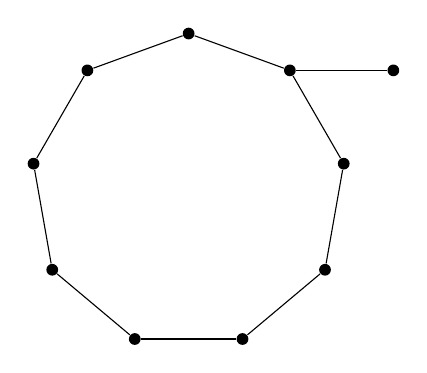
\begin{tikzpicture}
  [scale=2,auto=left,every node/.style={circle,inner sep=1.5pt, fill=black!100}]
  \node (n1) at (0.0000000,  1.0000000) {};
  \node(n2) at (0.6427876,  0.7660444)  {};
  \node (n3) at (0.9848078,  0.1736482)  {};
  \node (n4) at (0.8660254, -0.5000000) {};
  \node (n5) at (0.3420201, -0.9396926)  {};
  \node (n6) at (-0.3420201, -0.9396926)  {};
  \node (n7) at ( -0.8660254, -0.5000000) {};
  \node (n8) at (-0.9848078,  0.1736482)  {};
  \node (n9) at (-0.6427876,  0.7660444)  {};
  \node(n10) at (1.3,  0.7660444)  {};

  \foreach \from/\to in {n1/n2,n2/n3,n3/n4,n4/n5,n5/n6,n6/n7,n7/n8,n8/n9,n1/n9}
    \draw (\from) -- (\to);
    \draw (n2) -- (n10);
\end{tikzpicture}
\caption{An additional vertex and edge appended to $C_9$.}\label{fig:newgraph}
\end{center}
\end{figure}
\end{comment}

\begin{theorem}
Let $G$ be a graph consisting of $2n+2$ vertices and $2n+2$ edges such that $2n+1$ of them form a cycle and the remaining edge connects the remaining vertex to any existing vertex of the cycle. Further, let $I$ be the edge ideal of $G$ and let $L(t)$ and $D(t)$ retain their usual definitions with respect to $G$. Then $I^{(t)} = I^t + (D(t))$.
\end{theorem}
\begin{proof}
Without loss of generality, consider the cycle formed by $x_1, \ldots, x_{2n+1}$ with $e_{2n+2} = x_1 x_{2n+2}$ being the newly added edge. %Recall that $e_i = x_i x_{i+1}$ when $i \leq 2n$ and $e_{2n+1} = x_{2n+1} x_1$.

Let $m$ be a monomial expressed in optimal form $m = x_1^{a_1} x_2^{a_2} \cdots x_{2n+2}^{a_{2n+2}} e_1^{b_1} e_2^{b_2} \cdots e_{2n+2}^{b_{2n+2}}$, and recall that $b(m) = \sum b_i$.
As with the cycle, if $I^t = (L(t))$, it will follow that $I^{(t)} = I^t + (D(t))$.


%% For the forward containment, suppose $m \in I^t$. We know that given an arbitrary minimal vertex cover $V'$ and edge $e_j = x_j x_{j'}$ from $m$, it must be true that $x_j \in V'$ or $x_{j'} \in V'$ or both. Thus $w_{V'}(m) \geq b(m)$. Further, since $m \in I^t$, we know $b(m) \geq t$ and $\deg(m) \geq 2t$, which means that $m \in (L(t))$.

By Lemma \ref{lem:it sub lt} we know that $I^t \subseteq (L(t))$ so we must only show the reverse containment. Let $m\not\in I^t$ (which implies that $b(m) < t$). %, then we will show that $m\not\in (L(t))$. 
Lemma \ref{lem:m12 not in lt} allows us to consider only cases where $m$ either has multiple ancillaries or has a single ancillary of degree at least 2.
%% For the reverse containment, suppose that $m \not \in I^t$, so that $b(m) < t$, and
%Note that $\deg(m) \ge 2t$, else $m\notin (L(t))$ by definition.
We will construct a minimal vertex cover $V'$ of $G$ such that $w_{V'}(m) = b(m) < t$.
%% Observe that if $m$ has no ancillaries, then $2t\le \deg(m) = 2\sum b_i = 2b(m) < 2t$, a contradiction.
%% Additionally, if $m$ has exactly one ancillary factor with exponent equal to 1, we have $\deg(m) = 1 + 2b(m) < 1 + 2t$, and thus we may conclude $\deg(m) = 1+2b(m) < 2t$, a contradiction.
%% Thus, $m$ has at least one ancillary factor with exponent greater than 1, or two or more ancillary factors.


First, assume that $x_{2n+2}$ is the only ancillary of $m$, and observe that $a_{2n+2} \ge 2$. 
%In this case, as $b(m) < t$, we know that $a_{2n+2} \geq 2$ as $\deg(m) \geq 2t$. 
We may write $m$ as $m = x_{2n+2} e_1^{b_1} e_2^{b_2} \cdots e_{2n+2}^{b_{2n+2}} x_{2n+2}^{a_{2n+2} - 1}$. 
It cannot be true that $b_{i} \geq 1$ for all $i\in \{1,3,5,\ldots, 2n+1\}$, because it would then be possible to divide $m$ by some monomial $p = x_{2n+2} e_1 e_3\cdots e_{2n+1} x_{2n+2}$ which must be in optimal form by Lemma \ref{lem:splitm}; however, in this case, $p = e_{2n+2} e_2 e_4 \cdots e_{2n} e_{2n+2}$, contradicting that $p$ was in optimal form. 
Thus, at least one $b_{2j+1}$ is 0.
Then construct $V'$ as follows:

%\begin{enumerate}
%	\item If $b_1 = 0$, let $V' = \set{x_1, x_2, x_4, \ldots, x_{2n}}$. Then $w_{V'}(m) = b_1 + b_2 + \cdots b_{2n} = b(m) < t$.
%	\item If $b_{2j+1} = 0$ for some $j > 0$, let $V' = \set{x_{2j+1}, x_{2j+2}, x_{2j+4}, \ldots, x_{2n}, x_1, x_3, \ldots, x_{2j-1}}$.
%	Then $w_{V'}(m) = b_{2j+2} + b_{2j+4} + \cdots + b_{2n} + b_{2n+1} + b_1 + \cdots + b_{2j-2} + b_{2j-1} \le b(m) < t$.
%\end{enumerate}


\begin{enumerate}
    \item If $b_1 = 0$, %(which is a particular instance of our second case which is included for clarity) 
    let $$V' = \set{x_1, x_2, x_4, \ldots, x_{2n}}.$$ Then $w_{V'}(m) = (b_{2n+1}+b_{2n+2}+b_1) + (b_1+b_2) + (b_3+b_4) + \cdots + (b_{2n-1}+b_{2n}) = b_1 + \sum_{i=1}^{2n+2} b_i = 0 + \sum_{i=1}^{2n+2} b_i = b(m) < t$.
    \item If $b_{2j+1} = 0$ for some $j > 0$, let $$V' = \set{x_1, x_3, x_5, \ldots, x_{2j+1}, x_{2j+2}, x_{2j+4}, x_{2j+6}, \ldots, x_{2n}}.$$
     Then $w_{V'}(m) = (b_{2n+1}+b_{2n+2}+b_1) + (b_2+b_3) + \cdots + (x_{2j}+x_{2j+1}) + (x_{2j+1}+x_{2j+2}) + \cdots + (b_{2n-1}+b_{2n}) = b_{2j+1} + \sum_{i=1}^{2n+2} b_i = 0 + \sum_{i=1}^{2n+2} b_i = b(m) < t$.
\end{enumerate}



Now suppose that all ancillaries of $m$ are among the set $\set{x_1, x_2, \ldots, x_{2n+1}}$. %(we make no assumptions on whether or not $x__{2n+2}$ is ancillary).
By adapting the argument from Theorem \ref{lem:tl<it}, we may assume that there is either one ancillary with exponent at least 2, or that there are multiple ancillaries.
Use the construction in the proof of Theorem \ref{lem:tl<it} to decompose the subgraph $C_{2n+1}$ of $G$ as $H_1, H_2, \ldots, H_r$. % such that $x_1$ is a vertex in $H_1$.
Define $m_{C_{2n+1}} = x_1^{a_1} \cdots x_{2n+1}^{a_{2n+1}} e_1^{b_1} \cdots e_{2n+1}^{b_{2n+1}}$, i.e., $m_{C_{2n+1}} = m/(x_{2n+2}^{a_{2n+2}} e_{2n+2}^{b_{2n+2}})$.
The proof of Theorem \ref{lem:tl<it} provides minimal subcovers $S_1, S_2, \ldots, S_r$ such that $S = \cup S_q$ and $w_S(m_{C_{2n+1}}) = \sum_{i=1}^{2n+1} b_i$.

If $x_1\in S$, then $S$ covers $G$ and $w_S(m) = w_S(m_{C_{2n+1}}) + b_{2n+2} = \sum_{i=1}^{2n+2} b_i = b(m) < t$.
In this case, we may let $V' = S$.

On the other hand, if $x_1\notin S$, let $V' = S\cup \set{x_{2n+2}}$.
Then $w_{V'}(m) = w_S(m) + b_{2n+2} = \sum_{i=1}^{2n+2} b_i = b(m) < t$.





Next, assume that the ancillaries of $m$ are $x_{2n+2}$ and at least one $x_j$ in the cycle (where $j\ne 1$; if $j= 1$, we may write $x_{2n+2} x_1 = e_{2n+2}$, contradicting the assumption that $m$ is in optimal form). %such that $a_j = 1$.
%If $j$ is even, let $V' = \set{x_j, x_{j+2}, \cdots, x_{2n}, x_1, x_3, \cdots, x_{j-1}}$, and if $j$ is odd, let $V' = \set{x_j, x_{j+2} \cdots, x_{2n+1}, x_1, x_3, \cdots, x_{j-2}}$.
%In either case, $w_{V'}(m) = b(m) < t$.
%If $a_j > 1$ (or there are multiple ancillaries of $m$ in the cycle), 
Use the construction of Theorem \ref{lem:tl<it} to decompose the cycle into subgraphs $H_1, H_2, \ldots, H_r$ and note that $x_1$ is a vertex in $H_r$. 
Observe  that since $x_1$ is not ancillary, $x_1\notin H_i$ for any $i\ne r$.
Let the vertices of $H_i$ be represented by $\set{x_{\ell_{i}}, x_{\ell_{i}+1}, \ldots, x_{\ell_{i+1}}}$, where $x_{\ell_1}, \ldots, x_{\ell_r}$ are ancillaries, and we wrap around with $x_{\ell_{r+1}}$ representing $x_{\ell_1}$.
For all $i \ne r$, the proof of Theorem \ref{lem:tl<it} gives a construction of a minimal vertex subcover $S_i$ with the required properties.
Now construct a subgraph $H_r'$ of $G$ as follows: $V(H_r') = V(H_r) \cup \set{x_{2n+2}}$ and $E(H_r') = E_{H_r} \cup \set{\set{x_1, x_{2n+2}}}$.
Decompose $H_r'$ as two induced subgraphs $H_{r_a}'$ and $H_{r_b}'$ of $G$ on the vertices $\set{x_{\ell_r}, \ldots, x_1, x_{2n+2}}$ and $\set{x_{2n+2}, x_1, \ldots, x_{\ell_1}}$.
We observe that we may now use the construction in the proof of Theorem \ref{lem:tl<it} to build minimal covers of $H_{r_a}'$ and $H_{r_b}'$ containing $x_1$ (and not $x_{2n+2}$) whose union gives a cover $S_r$ of $H_r'$.
Given $m_r = x_{\ell_r}^{a_{\ell_r}} x_{\ell_{1}}^{a_{\ell_{1}}} x_{2n+2}^{a_{2n+2}} e_{\ell_r}^{b_{\ell_r}} e_{\ell_r+1}^{b_{\ell_r + 1}} \cdots e_{2n+2}^{b_{2n+2}} e_1^{b_1} \cdots e_{\ell_1-1}^{b_{\ell_1-1}}$, note that $w_{S_r'}(m_r) = b(m_r)$.
Then the union $V' = \cup_{i=1}^r S_i$ has the required property that $w_{V'}(m) = b(m)$.




In all cases, $m\notin L(t)$, and, by extension, $m\notin (L(t))$.

\end{proof}




We also verify that the answer to Question \ref{conj:anygraph} is positive when $G$ is a complete graph.
Thus, additional study is needed to identify the precise graph-theoretic property for which Question \ref{conj:anygraph} has an affirmative answer.

\begin{theorem}
  Let $R=k[x_1,\ldots,x_n]$ and let $K_n$ denote the complete graph on $\set{x_1,\ldots,x_n}$. 
  Further, let $I=I(K_n)$ and $L(t)$ and $D(t)$ maintain their definitions as above. Then $I^{(t)} = I^t + (D(t))$
%%  = (\{x^{\underline{a}} | x^{\underline{a}}\in R \text{ and} \deg(x^{\underline{a}}) \geq 2t \text{ and for all minimal vertex covers } V', \, w_{V'}(x^{\underline{a}}) \geq t\})$
\end{theorem}

\begin{proof}
  Let $e_{i,j}$ denote the edge between $x_i$ and $x_j$ such that $i<j$. %Note that while the notation is different, the concept of optimal form still applies. 
  We will show that $I^t = (L(t))$.
  By Lemma \ref{lem:it sub lt}, we must only show $(L(t))\subseteq I^t$.
  Let $m\not\in I^t$ (which implies that $b(m) < t$), and recall that Lemma \ref{lem:m12 not in lt} allows us to consider only cases where $m$ either has multiple ancillaries or has a single ancillary of at least degree 2. 
  Let $m=x_1^{a_1}\cdots x_n^{a_n}e_{1,2}^{b_{1,2}}\cdots e_{n-1,n}^{b_{n-1,n}}$ be in optimal form. Then $m$ has at most $1$ ancillary because if $x_i^{a_i}$ and $x_j^{a_j}$ were both ancillaries, then $m$ could be expressed as $$m=x_1^{a_1}\cdots x_i^{a_i-1}\cdots x_j^{a_j-1}\cdots x_n^{a_n}e_{1,2}^{b_{1,2}}e_{1,3}^{b_{1,3}}\cdots e_{i,j}^{b_{i,j}+1}\cdots e_{n-1,n}^{b_{n-1,n}}.$$ %for some $s$ 
  %because there is guaranteed to be an edge between $x_i$ and $x_j$ as $K_n$ is complete. 
  Thus $m$ has exactly $1$ ancillary and it must have a degree of at least 2.
  
  Without loss of generality, let $x_1^{a_1}$ be the ancillary of $m$. Note that $b_{i,j}=0$ if $i,j\not=1$. If this was not the case, $m$ could be expressed in a more optimal form as $$m=x_1^{a_1-2}\cdots x_n^{a_n}e_{1,2}^{b_{1,2}}e_{1,3}^{b_{1,3}}\cdots e_{1,i}^{b_{1,i}+1}\cdots e_{1,j}^{b_{1,j}+1}\cdots e_{i,j}^{b_{i,j}-1}\cdots e_{n-1,n}^{b_{n-1,n}}.$$
  Let $V' = \set{x_2,\ldots, x_n}$. 
  Observe that $V'$ covers $K_n$ and
\begin{align*}
  w_{v'}(m) &= w_{v'}(x_2^{b_{1,2}+b_{2,3}+b_{2,4}+\cdots+b_{2,n}} + x_3^{b_{1,3}+b_{2,3}+b_{3,4}+\cdots+b_{3,n}} + \cdots + x_n^{b_{1,n}+b_{2,n}+b_{3,n}+\cdots+b_{n-1,n}}) \\
  &= w_{v'}(x_2^{b_{1,2}+0+\cdots+0} + x_3^{b_{1,3}+0+\cdots+0} + \cdots + x_n^{b_{1,n}+0+\cdots+0}) \\
  &= \sum_{j=2}^n b_{1,j} \\
  &= \sum_{j=2}^n b_{1,j} + \sum_{i=2}^{n-1}\sum_{j=i+1}^n b_{i,j} \\
  &= \sum_{i=1}^{n-1}\sum_{j=i+1}^n b_{i,j} \\
  &= b(m).
\end{align*}
Thus $w_{v'}(m) = b(m) < t$, so $m \not\in L(t)$ and by the same argument, no divisor of $m$ is in $L(t)$, which means $m \not\in (L(t))$. 

Therefore, $I^t = (L(t))$. 
Because $I^{(t)} = (L(t)) + (D(t))$ by Corollary \ref{thm:sorta}, this leads to the desired result that $I^{(t)} = I^t + (D(t))$.
\end{proof}

\subsection*{Acknowledgements} This work was supported by Dordt College's summer undergraduate research program in the summer of 2017. All three authors wish to express deep gratitude to the Dordt College Office of Research and Scholarship for the opportunity to undertake this project.
The authors also wish to thank the referee for the many helpful comments on their work. In particular, the proof of Theorem \ref{thm:sdefects} was improved substantially by the referee's suggestions.


\bibliography{summer17.bib}{}
\bibliographystyle{plain}



\end{document}





\begin{comment}




We will use the approach of Theorem \ref{lem:tl<it}, which is to partition $G$ into trail subgraphs $H_0,H_1,\ldots, H_r$ using the ancillaries of $m$ as endpoints. 
We carry out the same process on this graph, with the only difference being that one of these subgraphs is not guaranteed to be a trail of vertices joined between a pair of (possibly distinct) ancillaries. 
In particular, the subgraph that includes $x_{2n+2}$ will be the only subgraph of $G$ that does not follow that pattern. 
For convenience and consistency in what follows, we let that subgraph be denoted as $H_0$.



We will consider in turn the following four cases.
\begin{itemize}
\item[] \begin{itemize}
\item[] \begin{itemize}
%\item[Case 0:  ] Both $x_{2n+2}$ and $x_{1}$ are ancillaries.
\item[Case 1:  ] Neither $x_1$ nor $x_{2n+2}$ are ancillaries.
\item[Case 2:  ] $x_1$ is an ancillary and $x_{2n+2}$ is not.
\item[Case 3:  ] $x_{2n+2}$ is an ancillary, $x_1$ is not, and there is at least one other ancillary.
\item[Case 4:  ] $x_{2n+2}$ is the only ancillary.
\end{itemize}
\end{itemize}
\end{itemize}

\noindent (Observe that we may not have both $x_1$ and $x_{2n+2}$ as ancillary in $m$, as their adjacency in $G$ would imply that $m$ is not in optimal form.)

Our goal is to prove that, in each case, it is possible to find some vertex cover of $G$ that has a vertex weight equal to the number of edges $b(m)$ in an optimal factorization of $m$, since it would follow that $m \not \in (L(t))$.
We will make repeated use of the construction in Theorem \ref{lem:tl<it} which demonstrates the existence of such a vertex cover on the odd cycle $C_{2n+1}\subseteq G$.
%Note that, in most cases, it will be sufficient to prove that $H_0$ can be covered by a set $S_0$ of vertices whose vertex weight restricted to $H_0$ is equal to the number of edges of $H_0$ appearing in the optimal factorization of $m$, because we already know that relationship for the $H_q$, $1\le i \le r$, as described in Theorem \ref{lem:tl<it}.
Further, we will only be concerned with monomials of degree at least $2t$, as no monomial of $(L(t))$ can have a degree less than $2t$. 

%\textbf{Case 0:} This case is not actually possible because no optimal factorization of a monomial can include two adjacent ancillaries.

\textbf{Case 1:} Observe that if there are no ancillaries, we have $2t \le \deg(m) = 2 \sum b_i = 2b(m) < 2t$.
Thus, there is at least one ancillary.
Use the method of Theorem \ref{lem:tl<it} to partition the subgraph $C_{2n+1}$ into paths along the ancillaries of $m$, and denote these paths by $H_1, H_2,\ldots, H_r$, where $x_1\in V_{H_1}$.
Then Theorem \ref{lem:tl<it} gives a minimal vertex cover $V'$ of $C_{2n+1}$ such that $w_{V'}(m) = b(m_{C_{2n+1}})$ , where $b(m_{C_{2n+1}})$ denotes the sum $\sum_{i=1}^{2n+1} b_i$.
If $x_1 \in V'$, we are done, as $V'$ minimally covers $G$ with the properties we require.
If $x_1\notin V'$, let $V'' = V'\cup \set{x_{2n+2}}$.
Then $w_{V''}(m) = w_{V'}(m) + b_{2n+2} = \sum_{i=1}^{2n+2} b_i = b(m)$.


%Suppose neither $x_1$ nor $x_{2n+2}$ are ancillary, and consider $C_{2n+1}$ as a subgraph of $G$. 
%If we partition $C_{2n+1}$ using the ancillaries from $m$, we can find some set of vertices $\mathcal{U} = \cup_{i\ge 1} S_q$, where $S_q$ minimally covers $H_q\setminus\set{x_{2n+2}}$. % that cover each subgraph, including the subgraph that has the same ancillary endpoints as $H_0$.
%Then $U_0$ will either include $x_1$, in which case this same set of vertices will be able to cover $H_0$ and have a vertex weight equal to the number of edges, or it will not include $x_1$, in which case adding $x_{2n+2}$ to $U_0$ will be able to cover $H_0$ and have a weight equal to the number of edges.

\textbf{Case 2:} Suppose $x_1$ is an ancillary and $x_{2n+2}$ is not.
Use $x_1$ to decompose $G$ into the graph $C_{2n+1}$ and the graph $H$ with vertex set $\set{x_1,x_{2n+2}}$ and edge set $E = \set{\set{x_1,x_{2n+2}}}$.
Apply the method of Theorem \ref{lem:tl<it} to $C_{2n+1}$ to obtain a minimal vertex cover $V'$ of $C_{2n+1}$ such that $w_{V'}(m) = b(m_{C_{2n+1}})$, and then set $V'' = V'\cup \set{x_{2n+2}}$.
We then have $w_{V''}(m) = w_{V'}(m) + b_{2n+2} = \sum_{i=1}^{2n+2} b_i = b(m)$.
%
%Since $x_1$ is an ancillary, it divides $G$ into two graphs, which are the cycle $C_{2n+1}$ and  The set $U_0$ containing just $x_{2n+2}$ fulfills all requirements.

\textbf{Case 3:} Suppose $x_1$ is not ancillary but $x_{2n+2}$ is, along with some other vertex $x_i$.
As before, use the method of Theorem \ref{lem:tl<it} to decompose $C_{2n+1}$ into a sequence of paths $H_1, H_2,\ldots, H_r$ along the ancillaries such that $x_1$ is a vertex of $H_1$.




Let the vertices of $H_1$ be $V_{H_1} = \{x_i, x_{i+1}, \ldots, x_{2n+1}, x_{2n+2}, x_1,x_2, \ldots, x_j\}$, where the only ancillaries of $m$ appearing in $H_1$ are $x_i, x_j$, and $x_{2n+2}$.
%
%When $x_{2n+2}$ is an ancillary and there is at least one other ancillary in $m$, we can define the vertices of $H_0$ as $V(H_0) = \{x_i, x_{i+1}, \ldots, x_{2n+1}, x_{2n+2}, x_1,x_2, \ldots, x_j\}$  where the only ancillaries of $H_0$ are $x_i$, $x_j$, and $x_{2n+2}$.
(Note that $x_i$ and $x_j$ may be the same vertex if there is only one other ancillary besides $x_{2n+2}$.)
Consider the paths from $x_i$ to $x_{2n+2}$ as the indices increase and $x_j$ to $x_{2n+2}$ as the indices decrease, which we shall refer to as $P_1$ and $P_2$ respectively.
Recall that for any path surrounded on both sides by ancillaries, Theorem \ref{lem:tl<it} demonstrates the existence of a vertex cover $S_q$ such that $w_{S_q}(m_{H_q}) = b(m_{H_q})$. %that has a weight equal to the sum of edge exponents for its respective monomial.
Further, note that each such cover will include the vertices adjacent to the ancillaries, regardless of how many vertices there are in the path.
Let $S_{P_1}$ be the minimal vertex cover for $P_1$ and $S_{P_2}$ be the minimal vertex cover for $P_2$ such that their vertex weights equal the sum of the edge exponents along each path.
As both $S_{P_1}$ and $S_{P_2}$ both contain $x_1$, it follows that the union $S_1 = S_{P_1} \cup S_{P_2}$ of these vertex covers minimally covers $H_1$.
Further, this cover has a weight equal to the sum of edge exponents in the subgraph.

\textbf{Case 4:} Finally, assume that $x_{2n+2}$ is the only ancillary of $m$.
In this case, as $b(m) < t$, we know that $a_{2n+2} \geq 2$ as $\deg(m) \geq 2t$.
Let us rewrite $m$ in an equally optimal form of $m = x_{2n+2} e_1^{b_1} e_2^{b_2} \cdots e_{2n+2}^{b_{2n+2}} x_{2n+2}^{a_{2n+2} - 1}$.
It cannot be true that $b_{i} \geq 1$ for all $i\in \{1,3,5,\ldots, 2n+1\}$, because it would then be possible to divide $m$ by some monomial $p = x_{2n+2} e_1 e_3\cdots e_{2n+1} x_{2n+2}$ which must be in optimal form by Lemma \ref{lem:splitm}; however, in this case, $p = e_{2n+2} e_2 e_4 \cdots e_{2n} e_{2n+2}$, contradicting that $p$ was in optimal form.
Thus, at least one $b_{2j+1} = 0$.
Construct $\mathcal{U}$ as follows:

\begin{enumerate}
	\item If $b_1 = 0$, let $\mathcal{U} = \set{x_1, x_2, x_4, \ldots, x_{2n}}$. Then $w_\mathcal{U}(m) = b_1 + b_2 + \cdots b_{2n} \le b(m) < t$.
	\item if $b_{2j+1} = 0$ for some $j > 0$, let $\mathcal{U} = \set{x_{2j+1}, x_{2j+2}, x_{2j+4}, \ldots, x_{2n}, x_1, x_3, \ldots, x_{2j-1}}$.
	Then $w_{\mathcal{U}}(m) = b_{2j+2} + b_{2j+4} + \cdots + b_{2n} + b_{2n+1} + b_1 + \cdots + b_{2j-2} + b_{2j-1} \le b(m) < t$.
\end{enumerate}

%Thus, if we begin with a pair of vertices that do not form an edge in $m$ and add alternating vertices thereafter to that set, we can find a set of vertices that cover $G$ without exceeding a weight of $b(m)$.

These  cases account for all possible combinations for $m$, and they all lead to the same conclusion: $m \not \in L(t)$.
%%%%
%Without loss of generality, consider the cycle formed by $x_1, \ldots, x_{2n+1}$ with $e_{2n+2} = x_1 x_{2n+2}$  the newly added edge. Recall that $e_i = x_i x_{i+1}$ when $i \leq 2n$ and $e_{2n+1} = x_{2n+1} x_1$.
%
%As before, our first step is to prove that $I^t \subseteq (L(t))$. This is straightforward, as the initial proof did not depend on $G$ being a cycle. Again, let $m \in I^t$ be a monomial expressed in optimal form $m = x_1^{a_1} x_2^{a_2} \cdots x_{2n+2}^{a_{2n+2}} e_1^{b_1} e_2^{b_2} \cdots e_{2n+2}^{b_{2n+2}}$, and recall that $b(m) = \sum b_i$. In order for $m$ to be an element of $I^t$, we know that $b(m) \geq t$ and $\deg(m) \geq 2t$. Given an arbitrary minimal vertex cover $V'$ and edge $e_j = x_j x_{j'}$ from $m$, it must be true that $x_j \in V'$ or $x_{j'} \in V'$ or both because every edge must have at least one of its vertices in any cover of $G$. This tells us that $w_{V'}(m) \geq b(m) \geq t$, and thus $m \in L(t)$. As both $I^t$ and $(L(t))$ are monomial ideals, this is sufficient to claim that $I^t \subseteq (L(t))$.
%
%For the reverse containment, suppose that there is some $m \not \in I^t$ such that $m$ can be expressed in optimal form $m = x_1^{a_1} x_2^{a_2} \cdots x_{2n+2}^{a_{2n+2}} e_1^{b_1} e_2^{b_2} \cdots e_{2n+2}^{b_{2n+2}}$. As before, we assume that $b(m) < t$.
%
%We will consider in turn the following five cases.
%\begin{itemize}
%\item[] \begin{itemize}
%\item[] \begin{itemize}
%\item[Case 0:  ] Both $x_{2n+2}$ and $x_{1}$ are ancillaries.
%\item[Case 1:  ] $x_{2n+2}$ is the only ancillary.
%\item[Case 2:  ] $x_{2n+2}$ is an ancillary, $x_1$ is not, and there is at least one other ancillary.
%\item[Case 3:  ] $x_1$ is an ancillary and $x_{2n+2}$ is not.
%\item[Case 4:  ] Neither $x_1$ nor $x_{2n+2}$ are ancillaries.
%\end{itemize}
%\end{itemize}
%\end{itemize}
%
%Recall that our approach to Theorem \ref{lem:tl<it} was to use the ancillaries to partition the graph into subgraphs with the ancillaries as endpoints.
%We will carry out a similar process on this graph, and all of the paths will have the same properties as before, except for the one subgraph that includes $x_{2n+2}$ which we shall refer to as $H_0$.

%Of course, $H_0$ does not contain just the one vertex, but rather every vertex up to and including the next closest ancillary or ancillaries.
%In addition, let $m'_{H_0}$ be the optimal monomial factorization that consists of the product of all ancillaries $x_i^{a_i}$ and edges $e_j^{b_j}$ of $H_0$. NOT TOTALLY CLEAR ON HOW $H_0$ IS DEFINED.
%
%Our goal is to demonstrate that for each case, there exists some vertex cover $S_{H_0}$ such that $w_{S_{H_0}}(m'_{H_0}) = b(m'_{H_0})$. Then we will conclude that there is some vertex cover of $G$ that has a weight less than $t$.
%Note that we will only be concerned with monomials of degree at least $2t$, as no monomial of degree less than $2t$ is in $I^t$.
%
%
%\textbf{Case 0:} Since $x_{2n+2}$ and $x_{1}$ are adjacent, it cannot actually be true that they are both ancillaries if $m'_{H_0}$ is in an optimal form. It would always be possible to form at least one more edge between them.
%
%\textbf{Case 1:} Since $x_{2n+2}$ is the only ancillary of $m$ and $b(m) < t$, we know that $a_{2n+2} \geq 2$ as $\deg(m) \geq 2t$. Rewrite $m$ optimally as $m = x_{2n+2} e_1^{b_1} e_2^{b_2} \cdots e_{2n+2}^{b_{2n+2}} x_{2n+2}^{a_{2n+2} - 1}$. Via Lemma \ref{lem:splitm}, we can see that it cannot be true that $b_{i} \geq 1$ for all $i$ in $\{1,3,5,\ldots, 2n+1\}$, because it would then be possible to divide $m$ by some monomial $p = x_{2n+2} e_1 e_3\cdots e_{2n+1} x_{2n+2} = e_{2n+2} e_2 e_4 \cdots e_{2n} e_{2n+2}$.
%Let $e_h$ be one of the edges with an exponent of 0 in $p$, and
%consider $S = \{x_1, x_3, \ldots, x_h, x_{h+1}, x_{h+3}, \ldots, x_{2n}\}$, which is a vertex cover for $G$. We know that the simplified form of $m$ is:
%
%\begin{align*}
%m &= x_{2n+2}^{a_{2n+2}} e_{1}^{b_{1}} e_{2}^{b_{2}}  \cdots e_{2n+1}^{b_{2n+1}} e_{2n+2}^{b_{2n+2}}\\
%&= x_{2n+2}^{a_{2n+2}} (x_{1} x_2)^{b_{1}} (x_{2} x_3)^{b_{2}} \cdots (x_{2n+1} x_{1})^{b_{2n+1}} (x_{2n+2} x_1)^{b_{2n+2}}\\
%&= x_1^{(b_1+b_{2n+1}+b_{2n+2})} x_{2}^{(b_{1} + b_{2})} x_{3}^{(b_{2} + b_{3})} \cdots x_{2n+1}^{(b_{2n} + b_{2n+1})} x_{2n}^{(b_{2n-1} + b_{2n})} x_{2n+2}^{(b_{2n+2} + a_{2n+2})}
%\end{align*}
%
%Thus:
%
%\begin{align*}
%w_{S}(m) &= (b_1+b_{2n+1}+b_{2n+2}) + (b_{2}+b_{3}) + \ldots + (b_{h-1}+b_{h}) \\
%&\hspace{1cm} + (b_{h} + b_{h+1}) + (b_{h+2} + b_{h+3}) + \ldots + (b_{2n-1}+b_{2n}) \\
%&= b_{i+2h+1} +  \sum\limits_{i = 1}^{2n+2} b_i\\
%&= b_{i+2h+1} + b(m) \\
%&= 0 + b(m) \\
%&= b(m)
%\end{align*}
%
%\textbf{Case 2:} Let $V(H_0) = \{x_i, x_{i+1}, \ldots, x_{2n+1}, x_{2n+2}, x_1,x_2 \ldots x_j\}$  where the only ancillaries are $x_i$, $x_j$, and $x_{2n+2}$. THIS ISN'T QUITE THE WAY CASE 2 IS STATED ABOVE. Consider the paths from $x_i$ to $x_{2n+2}$ and $x_j$ to $x_{2n+2}$, which we shall refer to as $P_1$ and $P_2$ respectively. Recall from our proof of Theorem \ref{lem:tl<it} that for any direct path surrounded on both sides by ancillaries, there exists some vertex cover that has a weight equal to the sum of edge exponents for its respective monomial. Further, note that each cover will include the vertices adjacent to the ancillaries, regardless of how many vertices there are in the path. Let $S_{P_1}$ be the vertex cover for $P_1$ and $S_{P_2}$ be the vertex cover for $P_2$ such that $w_{S_{P_1}}(m'_{P_1}) = b(m'_{P_1}) = \sum \limits_{h=i}^{2n+2} b_h$ and $w_{S_{P_2}}(m'_{P_2}) = b(m'_{P_2}) = b_{2n+2} + \sum \limits_{h=1}^{j} b_h$. Now let $S_{H_0} = S_{P_1} \cup S_{P_2}$. As both of the original covers had included $x_1$, once we delete the redundancies, which is actually just $b_{2n+2}$, we will see that the weight of this new cover is equal to the sum of the edge exponents as well.
%
%\textbf{Case 3:} When $x_1$ is an ancillary, it follows that $V(H_0) = \{x_1,x_{2n+2}\}$ and the only edge of $H_0$ is $e_{2n+2}$. As $x_{2n+2}$ is not an ancillary, we know that $m'_{H_0} = x_1^{(a_1+b_{2n+2})}x_{2n+2}^{b_{2n+2}}$. Further, if we let $S_{H_0} = \{x_{2n+2}\}$, we can see that $w_{S_{H_0}}(m'_{H_0}) = b_{2n+2} = b(m'_{H_0})$.
%
%\textbf{Case 4:} When neither $x_1$ nor $x_{2n+2}$ is an ancillary, consider the set of vertices $S_{H_0}$ that would have covered that string of vertices $H_0$ if it were not for $x_{2n+2}$ being added to the cycle. If we use the same method described in Theorem \ref{lem:tl<it} to find this set, we know that one of its vertex covers will have a weight equal to the number of edges in it. Now, suppose that $x_1 \in S_{H_0}$. Then, when we take $x_{2n+2}$ and $e_{2n+2}$ back into consideration, it will still be true that $w_{S_{H_0}}(m'_{H_0}) = b(m'_{H_0})$ because $e_{2n+2}$ is connected to $x_1$. Alternatively, suppose that $x_1 \not \in S_{H_0}$. Let $S'_{H_0} = S_{H_0} \cup \{x_{2n+2}\}$. Since $x_{2n+2}$ is not an ancillary, we know that $w_{S'_{H_0}}(m'_{H_0}) = b(m'_{H_0})$ because $S_{H_0}$ adequately covers all edges excluding $e_{2n+2}$, which is the only edge of $x_{2n+2}$.
%
%
%In Cases 2, 3, and 4, we have proven that there exists some $S_{H_0}$ such that $w_{S_{H_0}}(m'_{H_0}) = b(m'_{H_0})$. Recall that each remaining subgraph of $G$ is contained between a pair of ancillaries, which means that we are able to find vertex covers for each of them such that the weight is equal to the sum of edge exponents. Thus, if we find the union of $S_{H_0}$ and the other subgraphs' vertex covers, we can find some set of vertices $S$ that can adequately cover $G$, such that $w_{S}(m) = b(m)$. Similarly, in Case 1, we directly proved that there exists some $S$ such that $w_{S}(m) = b(m)$. Finally, since everything in Case 0 leads to a contradiction, we know that for any monomial $m \not \in I^t$ written in optimal form, there exists some $S$ where $w_{S}(m) = b(m)$.
%
%Since we know $b(m) < t$, it follows that $m \not \in L(t)$ and by extension $m \not \in (L(t))$.
\end{comment}
